\PassOptionsToPackage{unicode=true}{hyperref} % options for packages loaded elsewhere
\PassOptionsToPackage{hyphens}{url}
%
\documentclass[12pt,openright,oneside,a4paper,chapter=TITLE,section=TITLE,subsection=Title,english,french,spanish,portugues,sumario=tradicional]{04-class-files/abntex2}
\usepackage{lmodern}
\usepackage{amssymb,amsmath}
\usepackage{ifxetex,ifluatex}
\usepackage{fixltx2e} % provides \textsubscript
\ifnum 0\ifxetex 1\fi\ifluatex 1\fi=0 % if pdftex
  \usepackage[T1]{fontenc}
  \usepackage[utf8]{inputenc}
  \usepackage{textcomp} % provides euro and other symbols
\else % if luatex or xelatex
  \usepackage{unicode-math}
  \defaultfontfeatures{Ligatures=TeX,Scale=MatchLowercase}
\fi
% use upquote if available, for straight quotes in verbatim environments
\IfFileExists{upquote.sty}{\usepackage{upquote}}{}
% use microtype if available
\IfFileExists{microtype.sty}{%
\usepackage[]{microtype}
\UseMicrotypeSet[protrusion]{basicmath} % disable protrusion for tt fonts
}{}
\IfFileExists{parskip.sty}{%
\usepackage{parskip}
}{% else
\setlength{\parindent}{0pt}
\setlength{\parskip}{6pt plus 2pt minus 1pt}
}
\usepackage{hyperref}
\hypersetup{
            pdfauthor={Nome do Discente},
            pdfborder={0 0 0},
            breaklinks=true}
\urlstyle{same}  % don't use monospace font for urls
\usepackage{color}
\usepackage{fancyvrb}
\newcommand{\VerbBar}{|}
\newcommand{\VERB}{\Verb[commandchars=\\\{\}]}
\DefineVerbatimEnvironment{Highlighting}{Verbatim}{commandchars=\\\{\}}
% Add ',fontsize=\small' for more characters per line
\usepackage{framed}
\definecolor{shadecolor}{RGB}{248,248,248}
\newenvironment{Shaded}{\begin{snugshade}}{\end{snugshade}}
\newcommand{\AlertTok}[1]{\textcolor[rgb]{0.94,0.16,0.16}{#1}}
\newcommand{\AnnotationTok}[1]{\textcolor[rgb]{0.56,0.35,0.01}{\textbf{\textit{#1}}}}
\newcommand{\AttributeTok}[1]{\textcolor[rgb]{0.77,0.63,0.00}{#1}}
\newcommand{\BaseNTok}[1]{\textcolor[rgb]{0.00,0.00,0.81}{#1}}
\newcommand{\BuiltInTok}[1]{#1}
\newcommand{\CharTok}[1]{\textcolor[rgb]{0.31,0.60,0.02}{#1}}
\newcommand{\CommentTok}[1]{\textcolor[rgb]{0.56,0.35,0.01}{\textit{#1}}}
\newcommand{\CommentVarTok}[1]{\textcolor[rgb]{0.56,0.35,0.01}{\textbf{\textit{#1}}}}
\newcommand{\ConstantTok}[1]{\textcolor[rgb]{0.00,0.00,0.00}{#1}}
\newcommand{\ControlFlowTok}[1]{\textcolor[rgb]{0.13,0.29,0.53}{\textbf{#1}}}
\newcommand{\DataTypeTok}[1]{\textcolor[rgb]{0.13,0.29,0.53}{#1}}
\newcommand{\DecValTok}[1]{\textcolor[rgb]{0.00,0.00,0.81}{#1}}
\newcommand{\DocumentationTok}[1]{\textcolor[rgb]{0.56,0.35,0.01}{\textbf{\textit{#1}}}}
\newcommand{\ErrorTok}[1]{\textcolor[rgb]{0.64,0.00,0.00}{\textbf{#1}}}
\newcommand{\ExtensionTok}[1]{#1}
\newcommand{\FloatTok}[1]{\textcolor[rgb]{0.00,0.00,0.81}{#1}}
\newcommand{\FunctionTok}[1]{\textcolor[rgb]{0.00,0.00,0.00}{#1}}
\newcommand{\ImportTok}[1]{#1}
\newcommand{\InformationTok}[1]{\textcolor[rgb]{0.56,0.35,0.01}{\textbf{\textit{#1}}}}
\newcommand{\KeywordTok}[1]{\textcolor[rgb]{0.13,0.29,0.53}{\textbf{#1}}}
\newcommand{\NormalTok}[1]{#1}
\newcommand{\OperatorTok}[1]{\textcolor[rgb]{0.81,0.36,0.00}{\textbf{#1}}}
\newcommand{\OtherTok}[1]{\textcolor[rgb]{0.56,0.35,0.01}{#1}}
\newcommand{\PreprocessorTok}[1]{\textcolor[rgb]{0.56,0.35,0.01}{\textit{#1}}}
\newcommand{\RegionMarkerTok}[1]{#1}
\newcommand{\SpecialCharTok}[1]{\textcolor[rgb]{0.00,0.00,0.00}{#1}}
\newcommand{\SpecialStringTok}[1]{\textcolor[rgb]{0.31,0.60,0.02}{#1}}
\newcommand{\StringTok}[1]{\textcolor[rgb]{0.31,0.60,0.02}{#1}}
\newcommand{\VariableTok}[1]{\textcolor[rgb]{0.00,0.00,0.00}{#1}}
\newcommand{\VerbatimStringTok}[1]{\textcolor[rgb]{0.31,0.60,0.02}{#1}}
\newcommand{\WarningTok}[1]{\textcolor[rgb]{0.56,0.35,0.01}{\textbf{\textit{#1}}}}
\usepackage{longtable,booktabs}
% Fix footnotes in tables (requires footnote package)
\IfFileExists{footnote.sty}{\usepackage{footnote}\makesavenoteenv{longtable}}{}
\usepackage{graphicx,grffile}
\makeatletter
\def\maxwidth{\ifdim\Gin@nat@width>\linewidth\linewidth\else\Gin@nat@width\fi}
\def\maxheight{\ifdim\Gin@nat@height>\textheight\textheight\else\Gin@nat@height\fi}
\makeatother
% Scale images if necessary, so that they will not overflow the page
% margins by default, and it is still possible to overwrite the defaults
% using explicit options in \includegraphics[width, height, ...]{}
\setkeys{Gin}{width=\maxwidth,height=\maxheight,keepaspectratio}
\setlength{\emergencystretch}{3em}  % prevent overfull lines
\providecommand{\tightlist}{%
  \setlength{\itemsep}{0pt}\setlength{\parskip}{0pt}}
\setcounter{secnumdepth}{5}
% Redefines (sub)paragraphs to behave more like sections
\ifx\paragraph\undefined\else
\let\oldparagraph\paragraph
\renewcommand{\paragraph}[1]{\oldparagraph{#1}\mbox{}}
\fi
\ifx\subparagraph\undefined\else
\let\oldsubparagraph\subparagraph
\renewcommand{\subparagraph}[1]{\oldsubparagraph{#1}\mbox{}}
\fi

% set default figure placement to htbp
\makeatletter
\def\fps@figure{htbp}
\makeatother

%%%%%%%%%%%%%%%%%%%%%%%%%%%%%%%%%%%%%%%%%%%%%%%%%%%%%%%
% Arquivo para entrada de dados para a parte pré textual
%%%%%%%%%%%%%%%%%%%%%%%%%%%%%%%%%%%%%%%%%%%%%%%%%%%%%%%
% 
% Basta digitar as informações indicidas, no formato 
% apresentado.
%
%%%%%%%
% Os dados solicitados são, na ordem:
%
% tipo do trabalho
% componentes do trabalho 
% título do trabalho
% nome do autor
% local 
% data (ano com 4 dígitos)
% orientador(a)
% coorientador(a)(as)(es)
% arquivo com dados bibliográficos
% instituição
% setor
% programa de pós gradução
% curso
% preambulo
% data defesa
% CDU
% errata
% assinaturas - termo de aprovação
% resumos & palavras chave
% agradecimentos
% dedicatoria
% epígrafe


% Informações de dados para CAPA e FOLHA DE ROSTO
%----------------------------------------------------------------------------- 
\tipotrabalho{Trabalho Acadêmico}
%    {Relatório Técnico}
%    {Dissertação}
%    {Tese}
%    {Monografia}

% Marcar Sim para as partes que irão compor o documento pdf
%----------------------------------------------------------------------------- 
 \providecommand{\terCapa}{Sim}
 \providecommand{\terFolhaRosto}{Sim}
 \providecommand{\terTermoAprovacao}{Sim}
 \providecommand{\terDedicatoria}{Sim}
 \providecommand{\terFichaCatalografica}{Sim}
 \providecommand{\terEpigrafe}{Sim}
 \providecommand{\terAgradecimentos}{Sim}
 \providecommand{\terErrata}{Sim}
 \providecommand{\terListaFiguras}{Sim}
 \providecommand{\terListaTabelas}{Nao}
 \providecommand{\terSiglasAbrev}{Nao}
 \providecommand{\terResumos}{Sim}
 \providecommand{\terSumario}{Sim}
 \providecommand{\terAnexo}{Sim}
 \providecommand{\terApendice}{Sim}
 \providecommand{\terIndiceR}{Nao}
%----------------------------------------------------------------------------- 

\titulo{Modelode Trabalho Acadêmico em Rmarkdown baseado em modelo canônico \abnTeX adaptado para a UFPR}
\autor{}
\local{Curitiba}
\data{2020} %Apenas ano 4 dígitos

% Orientador ou Orientadora
\orientador{Prof. Dr. }
%Prof Emílio Eiji Kavamura, MSc}
\orientadora{
Prof\textordfeminine~Grace Kelly, DSc}
% Pode haver apenas uma orientadora ou um orientador
% Se houver os dois prevalece o feminino.

% Em termos de coorientação, podem haver até quatro neste modelo
% Sendo 2 mulhere e 2 homens.
% Coorientador ou Coorientadora
\coorientador{Prof. Dr. }%Prof Morgan Freeman, DSc}
\coorientadora{Prof\textordfeminine~Audrey Hepburn, DEng}

% Segundo Coorientador ou Segunda Coorientadora
\scoorientador{}
%Prof Jack Nicholson, DEng}
\scoorientadora{}
%Prof\textordfeminine~Ingrid Bergman, DEng}
% ----------------------------------------------------------
%\addbibresource{referencias}

% ----------------------------------------------------------
\instituicao{Universidade Federal do Paraná}

\def \ImprimirSetor{}%
%Setor de Tecnologia}

\def \ImprimirProgramaPos{Nome do programa ou departamento}

\def \ImprimirCurso{Nome do Curso}

\preambulo{
Trabalho apresentado como requisito parcial para a obtenção do título de (Título da formação) em (Nome do Curso ou Departamento) do  Nome do Setor da Universidade Federal do Paraná}
%do grau de Bacharel em Expressão Gráfica no curso de Expressão Gráfica, Setor de Exatas da Universidade Federal do Paraná}

%----------------------------------------------------------------------------- 

\newcommand{\imprimirCurso}{}
%Programa de P\'os Gradua\c{c}\~ao em Engenharia da Constru\c{c}\~ao Civil}

\newcommand{\imprimirDataDefesa}{
09 de Dezembro de 2018}

\newcommand{\imprimircdu}{
02:141:005.7}

% ----------------------------------------------------------
\newcommand{\imprimirerrata}{
Elemento opcional da \cites[4.2.1.2]{NBR14724:2011}. Exemplo:

\vspace{\onelineskip}

FERRIGNO, C. R. A. \textbf{Tratamento de neoplasias ósseas apendiculares com
reimplantação de enxerto ósseo autólogo autoclavado associado ao plasma
rico em plaquetas}: estudo crítico na cirurgia de preservação de membro em
cães. 2011. 128 f. Tese (Livre-Docência) - Faculdade de Medicina Veterinária e
Zootecnia, Universidade de São Paulo, São Paulo, 2011.

\begin{table}[htb]
\center
\footnotesize
\begin{tabular}{|p{1.4cm}|p{1cm}|p{3cm}|p{3cm}|}
  \hline
   \textbf{Folha} & \textbf{Linha}  & \textbf{Onde se lê}  & \textbf{Leia-se}  \\
    \hline
    1 & 10 & auto-conclavo & autoconclavo\\
   \hline
\end{tabular}
\end{table}}

% Comandos de dados - Data da apresentação
\providecommand{\imprimirdataapresentacaoRotulo}{}
\providecommand{\imprimirdataapresentacao}{}
\newcommand{\dataapresentacao}[2][\dataapresentacaoname]{\renewcommand{\dataapresentacao}{#2}}

% Comandos de dados - Nome do Curso
\providecommand{\imprimirnomedocursoRotulo}{}
\providecommand{\imprimirnomedocurso}{}
\newcommand{\nomedocurso}[2][\nomedocursoname]
  {\renewcommand{\imprimirnomedocursoRotulo}{#1}
\renewcommand{\imprimirnomedocurso}{#2}}


% ----------------------------------------------------------
\newcommand{\AssinaAprovacao}{

\assinatura{%\textbf
   {Professora} \\ UFPR}
   \assinatura{%\textbf
   {Professora} \\ ENSEADE}
   \assinatura{%\textbf
   {Professora} \\ TIT}
   %\assinatura{%\textbf{Professor} \\ Convidado 4}
      
   \begin{center}
    \vspace*{0.5cm}
    %{\large\imprimirlocal}
    %\par
    %{\large\imprimirdata}
    \imprimirlocal, \imprimirDataDefesa.
    \vspace*{1cm}
  \end{center}
  }
  
% ----------------------------------------------------------
%\newcommand{\Errata}{%\color{blue}
%Elemento opcional da \textcite[4.2.1.2]{NBR14724:2011}. Exemplo:
%}

% ----------------------------------------------------------
\newcommand{\EpigrafeTexto}{%\color{blue}
\textit{``Não vos amoldeis às estruturas deste mundo, \\
		mas transformai-vos pela renovação da mente, \\
		a fim de distinguir qual é a vontade de Deus: \\
		o que é bom, o que Lhe é agradável, o que é perfeito.\\
		(Bíblia Sagrada, Romanos 12, 2)}
}

% ----------------------------------------------------------
\newcommand{\ResumoTexto}{%\color{blue}
Segundo a \textcite[3.1-3.2]{abntex2modelo}, o resumo deve ressaltar o  objetivo, o método, os resultados e as conclusões do documento. A ordem e a extensão destes itens dependem do tipo de resumo (informativo ou indicativo) e do tratamento que cada item recebe no documento original. O resumo deve ser precedido da referência do documento, com exceção do resumo inserido no próprio documento. (\ldots) As palavras-chave devem figurar logo abaixo do  resumo, antecedidas da expressão Palavras-chave:, separadas entre si por ponto e finalizadas também por ponto.
}

\newcommand{\PalavraschaveTexto}{%\color{blue}
latex. abntex. editoração de texto.}

% ----------------------------------------------------------
\newcommand{\AbstractTexto}{%\color{blue}
This is the english abstract.
}
% ---
\newcommand{\KeywordsTexto}{%\color{blue}
latex. abntex. text editoration.
}

% ----------------------------------------------------------
\newcommand{\Resume}
{%\color{blue}
Il s'agit d'un résumé en français.
} 
% ---
\newcommand{\Motscles}
{%\color{blue}
 latex. abntex. publication de textes.
}

% ----------------------------------------------------------
\newcommand{\Resumen}
{%\color{blue}
Este es el resumen en español.
}
% ---
\newcommand{\Palabrasclave}
{%\color{blue}
latex. abntex. publicación de textos.
}

% ----------------------------------------------------------
\newcommand{\AgradecimentosTexto}{%\color{blue}
Os agradecimentos principais são direcionados à Gerald Weber, Miguel Frasson, Leslie H. Watter, Bruno Parente Lima, Flávio de  Vasconcellos Corrêa, Otavio Real Salvador, Renato Machnievscz\footnote{Os nomes dos integrantes do primeiro
projeto abn\TeX\ foram extraídos de \url{http://codigolivre.org.br/projects/abntex/}} e todos aqueles que contribuíram para que a produção de trabalhos acadêmicos conforme as normas ABNT com \LaTeX\ fosse possível.

Agradecimentos especiais são direcionados ao Centro de Pesquisa em Arquitetura da Informação\footnote{\url{http://www.cpai.unb.br/}} da Universidade de Brasília (CPAI), ao grupo de usuários
\emph{latex-br}\footnote{\url{http://groups.google.com/group/latex-br}} e aos novos voluntários do grupo \emph{\abnTeX}\footnote{\url{http://groups.google.com/group/abntex2} e
\url{http://abntex2.googlecode.com/}}~que contribuíram e que ainda
contribuirão para a evolução do \abnTeX.

Os agradecimentos principais são direcionados à Gerald Weber, Miguel Frasson, Leslie H. Watter, Bruno Parente Lima, Flávio de Vasconcellos Corrêa, Otavio Real Salvador, Renato Machnievscz\footnote{Os nomes dos integrantes do primeiro
projeto abn\TeX\ foram extraídos de \url{http://codigolivre.org.br/projects/abntex/}} e todos aqueles que contribuíram para que a produção de trabalhos acadêmicos conforme as normas ABNT com \LaTeX\ fosse possível.
}

% ----------------------------------------------------------
\newcommand{\DedicatoriaTexto}{%\color{blue}
\textit{ Este trabalho é dedicado às crianças adultas que,\\
   quando pequenas, sonharam em se tornar cientistas.}
	}


% Pacotes básicos 
% ----------------------------------------------------------
%\usepackage{lmodern}			% Usa a fonte Latin Modern			
\usepackage[utf8]{inputenc}		% Codificacao do documento (conversão automática dos acentos)
\usepackage{csquotes}
\usepackage[T1]{fontenc}		% Selecao de codigos de fonte.
\usepackage{lastpage}			% Usado pela Ficha catalográfica
\usepackage{indentfirst}		% Indenta o primeiro parágrafo de cada seção.
\usepackage{color}		    	% Controle das cores
\usepackage{graphicx}			% Inclusão de gráficos
\usepackage{microtype} 			% para melhorias de justificação
\usepackage{ifthen}		    	% para montar condicionais
%\usepackage[brazil]{babel}		% para utilizar termos em portugues
\usepackage[final]{pdfpages}    % para incluir páginas de arquivos pdf
\usepackage{lipsum}				% para geração de dummy text
\usepackage{csquotes}

%\usepackage[style=long]{glossaries}
%\usepackage{abntex2glossaries}

% permite representar o cancelamento de termos em texto ou equacoes
\usepackage{cancel} 		
% cores extendidas
\usepackage{xcolor} 		
% gera diagramas a partir de listas
\usepackage{smartdiagram}   
% Para a figura ficar na posição correta
\usepackage{float} 		    
% supporte para fontes da Text Companion 
\usepackage{textcomp} 		
% uso de longtable
\usepackage{longtable}		
% simbolos matematicos
\usepackage{amsmath}	
% páginas em paisagem
\usepackage{lscape}
% mescla de colunas em tabelas
\usepackage{multicol}
% mescla de linhas em tabelas
\usepackage{multirow}
% criação do indice de quadros
\usepackage{newfloat} 
% configura legenda 
\usepackage{caption} 		
%[format=plain]
	%\renewcommand\caption[1]{%
    \captionsetup{font=small}	% tamanho da fonte 10pt
    %,format=hang
 	% \caption{#1}}
	%\captionsetup{width=0.8\textwidth}

% Pacotes de citações BibLaTeX
% ----------------------------------------------------------
\usepackage[style=abnt,backref=true,backend=biber,citecounter=true,backrefstyle=three]{biblatex}


\DefineBibliographyStrings{brazil}{%
 backrefpage = {Citado \arabic{citecounter} vez na página},% originally "cited on page"
 backrefpages = {Citado \arabic{citecounter} vezes nas páginas},% originally "cited on pages"
}

% ----------------------------------------------------------

% alterando o aspecto da cor azul
\definecolor{blue}{RGB}{55,10,249}

% ----------------------------------------------------------
\PrepareListOf{quadro}{%
\renewcommand{\cftfigpresnum}{Quadro~}}

\DeclareFloatingEnvironment[
fileext=loq,
listname={\textbf{LISTA DE QUADROS}},
name=Quadro,
%placement=p,
within= none, % numeracao continua
%within=section, % numeracao reinicia em cada seccao
%chapterlistsgaps=off
]{quadro}

\newlistentry{quadro}{loq}{0}


% Customize ‘List of Diagrams’
\PrepareListOf{quadro}{%
\renewcommand{\cftquadropresnum}{\normalsize{QUADRO}~}
\setlength{\cftquadronumwidth}{3.2cm}
%\renewcommand{\cftquadroname}{\quadroname\space} 
\renewcommand*{\cftquadroaftersnum}{\hfill--\hfill}
}

\makeatletter
%% we define a helper macro for adjusting lists of new floats to
%% accept a * behind them for not being shown in the TOC, like
%% the other list printing commands in memoir
\newcommand{\AdjustForMemoir}[1]{%
  \csletcs{kept@listof#1}{listof#1}%
  \csdef{listof#1}{%
    \@ifstar
     {\csappto{newfloat@listof#1@hook}{\append@star}%
      \csuse{kept@listof#1}}%
     {\csuse{kept@listof#1}}%
  }
}
\def\append@star#1{#1*}
\makeatother


\AdjustForMemoir{quadro} % prepare `\listofdirfigures` so it accepts a *

\makeatletter
\let\oldcontentsline\contentsline
\def\contentsline#1#2{%
    \expandafter\ifx\csname l@#1\endcsname\l@section
	\expandafter\@firstoftwo
	\else
	\expandafter\@secondoftwo
	\fi
	{%
		\oldcontentsline{#1}{\MakeTextUppercase{#2}}%
	}{%
	\normalsize %ajusta tamanho da fonte na lista
	\oldcontentsline{#1}{#2}%
}%
}
\makeatother

% Ajusta indentação de Referencias no ToC
% ----------------------------------------------------------
\defbibheading{bay}[\bibname]{%
  \chapter*{#1}%
  \markboth{#1}{#1}%
  \addcontentsline{toc}{chapter}
  {\protect\numberline{}\bibname}
}

\makeatletter
\pretocmd{\chapter}{\addtocontents{toc}{\protect\addvspace{-5\p@}}}{}{}
\pretocmd{\section}{\addtocontents{toc}{\protect\addvspace{2\p@}}}{}{}
\makeatother
\makeindex
\usepackage{helvet}
\renewcommand{\familydefault}{\sfdefault}
\DeclareUnicodeCharacter{0301}{*}
\usepackage[style=abnt,]{biblatex}
\addbibresource{10-references/referencias.bib}

\author{Nome do Discente}
\date{2020}

\begin{document}

\ifthenelse{\equal{\terCapa}{Sim}}{
\imprimircapa}{}

\imprimirfolhaderosto*

\ifthenelse{\equal{\terFichaCatalografica}{Sim}}
 {\insereFichaCatalografica{}\cleardoublepage}
 {}

\ifthenelse{\equal{\terErrata}{Sim}}
 {\begin{errata}%\color{blue}
   \imprimirerrata
  \end{errata}}
 {}

\ifthenelse{\equal{\terTermoAprovacao}{Sim}}{
\insereAprovacao}{}

\ifthenelse{\equal{\terDedicatoria}{Sim}}{
\begin{dedicatoria}
   \vspace*{\fill}
   \centering
   \noindent
   \DedicatoriaTexto
   \vspace*{\fill}
\end{dedicatoria}
}{}

\ifthenelse{\equal{\terAgradecimentos}{Sim}}
 {\begin{agradecimentos}
    \AgradecimentosTexto
  \end{agradecimentos}
  }{}

\ifthenelse{\equal{\terEpigrafe}{Sim}}{
\begin{epigrafe}
    \vspace*{\fill}
	\begin{flushright}
        \EpigrafeTexto
	\end{flushright}
\end{epigrafe}
}{}

\ifthenelse{\equal{\terResumos}{Sim}}{
\begin{resumo}
    \ResumoTexto
    

   \noindent 
   \textbf{Palavras-chaves}: \PalavraschaveTexto
\end{resumo}

\begin{resumo}[ABSTRACT]
 \begin{otherlanguage*}{english}
   \AbstractTexto
   
   \noindent 
   \textbf{Key-words}: \KeywordsTexto
 \end{otherlanguage*}
\end{resumo}



\ifthenelse{\equal{\Resume}{}}
{}
{
 \begin{resumo}[RESUME]%Résumé
  \begin{otherlanguage*}{french}
     \Resume
     
   \noindent      
    \textbf{Mots clés}: \Motscles
  \end{otherlanguage*}
 \end{resumo}
} 


\ifthenelse{\equal{\Resume}{}}{}
{ \begin{resumo}[RESUMEN]
  \begin{otherlanguage*}{spanish}
    \Resumen 
   
   \noindent    
    \textbf{Palabras clave}: \Palabrasclave
  \end{otherlanguage*}
 \end{resumo}
}
}{}

\ifthenelse{\equal{\terListaFiguras}{Sim}}{
\pdfbookmark[0]{\listfigurename}{lof}
\listoffigures*
\cleardoublepage
}{}

\ifthenelse{\equal{\terListaTabelas}{Sim}}{
\listoftables*
\cleardoublepage
}{}

\ifthenelse{\equal{\terSiglasAbrev}{Sim}}{
    \imprimirlistadesiglas
    \cleardoublepage
    \imprimirlistadesimbolos
    \cleardoublepage
 }{}

\ifthenelse{\equal{\terSumario}{Sim}}{
\tableofcontents*
}{}

\textual

\pagestyle{simple}

\chapter[INTRODUÇÃO]{INTRODUÇÃO}

Este projeto é uma adaptação para o ambiente R Markdown utilizando a ferramenta bookdown combinando o modelo canônico de trabalho acadêmicos da \abnTeX e a adapatação para UFPR realizada por Emilio E Kawamura.

Nesse sentido esse documento de exemplo conterá as redações idendicas destes dois trabalhos, com acréscimo de exemplos de utilização e visualização de códigos em linguagem R.

Este documento e seu código-fonte são exemplos de referência de uso da classe
\textcite{abntex2} e do pacote \textcite{abntex2cite}. O documento
exemplifica a elaboração de trabalho acadêmico (tese, dissertação e outros do
gênero) produzido conforme a ABNT NBR 14724:2011 \emph{Informação e documentação
- Trabalhos acadêmicos - Apresentação}.

A expressão ``Modelo Canônico'' é utilizada para indicar que \abnTeX~não é
modelo específico de nenhuma universidade ou instituição, mas que implementa tão
somente os requisitos das normas da ABNT. Uma lista completa das normas
observadas pelo \abnTeX~é apresentada em \textcite{abntex2classe}.

Sinta-se convidado a participar do projeto \abnTeX! Acesse o site do projeto em
\url{http://www.abntex.net.br/}. Também fique livre para conhecer,
estudar, alterar e redistribuir o trabalho do \abnTeX, desde que os arquivos
modificados tenham seus nomes alterados e que os créditos sejam dados aos
autores originais, nos termos da ``The \LaTeX~Project Public
License''\footnote{\url{http://www.latex-project.org/lppl.txt}}.

Encorajamos que sejam realizadas customizações específicas deste exemplo para
universidades e outras instituições --- como capas, folha de aprovação, etc.
Porém, recomendamos que ao invés de se alterar diretamente os arquivos do
\abnTeX, distribua-se arquivos com as respectivas customizações.
Isso permite que futuras versões do \abnTeX\textasciitilde{}não se tornem automaticamente
incompatíveis com as customizações promovidas.

Este documento deve ser utilizado como complemento dos manuais do \abnTeX~
\cite{abntex2classe,abntex2cite,abntex2cite-alf} e da classe \textcite{memoir}
\cite{memoir}.

Esperamos, sinceramente, que o \abnTeX~aprimore a qualidade do trabalho que
você produzirá, de modo que o principal esforço seja concentrado no principal:
na contribuição científica.

Equipe \abnTeX 

Lauro César Araujo

Para obter os melhores resultados, compile este modelo usando a seguinte sequência de passos:

\begin{quote}
\begin{footnotesize}
\begin{verbatim}
pdflatex  main          // compilação inicial
bibtex main             // processa referências bibliográficas
pdflatex  main          // compilação final
\end{verbatim}
\end{footnotesize}
\end{quote}

ou

\begin{quote}
\begin{footnotesize}
\begin{verbatim}
make                    // faz tudo...
\end{verbatim}
\end{footnotesize}
\end{quote}

Os principais itens considerados na formatação deste documento foram:

\begin{itemize}

\item Papel em formato A4, com margens de 20 mm à direita e embaixo, 30 mm nos demais lados. Não devem ser usados cabeçalhos ou rodapés além dos que estão aqui propostos.

\item O texto principal do documento escrito em 12 pontos. O fonte principal do texto pode ser selecionado no arquivo \verb#packages.tex#.

\item Código-fonte, listagens e textos similares são formatados em fonte Courier 12 ou 10 pontos.

\item O espaçamento padrão entre linhas é 1,5 linhas (1 linha na versão final). Não inserir espaços adicionais entre parágrafos normais. Figuras, tabelas, listagens e listas de itens devem ter um espaço adicional antes e após os mesmos.

\item As páginas iniciais não são numeradas.

\item O corpo do texto é numerado com algarismos arábicos (1, 2, 3, ...) a partir da introdução, ate o final do documento. Os números de página devem estar situados no alto à direita (páginas direitas) ou à esquerda (páginas esquerdas).

\item Expressões em inglês, grego, latim ou outras línguas devem ser enfatizadas em itálico, como \emph{sui generis} ou \emph{scheduling} (use o comando \verb#\emph{...}#).

\item Para reforçar algo, deve-se usar somente \textbf{negrito}. \underline{Sublinhado} ou MAIÚSCULAS não devem ser usados como forma de ênfase!

\item As notas de rodapé também têm um modelo\footnote{As notas de rodapé dever ser escritas em tamanho 10 pt, numeradas em arábico.}. Notas de rodapé servem para fazer algum comentário paralelo; não as use para colocar URLs, referências bibliográficas ou significado de siglas.

\end{itemize}

Felizmente o \LaTeX~resolve a maior parte dessas questões!

\part{Referenciais teóricos}

\chapter{Lorem ipsum dolor sit amet}

\section{Aliquam vestibulum fringilla lorem}

\lipsum[1]

\lipsum[2-3]

\part{Preparação da pesquisa}

%% abtex2-modelo-include-comandos.tex, v-1.9.7 laurocesar
%% Copyright 2012-2018 by abnTeX2 group at http://www.abntex.net.br/ 
%%
%% This work may be distributed and/or modified under the
%% conditions of the LaTeX Project Public License, either version 1.3
%% of this license or (at your option) any later version.
%% The latest version of this license is in
%%   http://www.latex-project.org/lppl.txt
%% and version 1.3 or later is part of all distributions of LaTeX
%% version 2005/12/01 or later.
%%
%% This work has the LPPL maintenance status `maintained'.
%% 
%% The Current Maintainer of this work is the abnTeX2 team, led
%% by Lauro César Araujo. Further information are available on 
%% http://www.abntex.net.br/
%%
%% This work consists of the files abntex2-modelo-include-comandos.tex
%% and abntex2-modelo-img-marca.pdf
%%

% ---
% Este capítulo, utilizado por diferentes exemplos do abnTeX2, ilustra o uso de
% comandos do abnTeX2 e de LaTeX.
% ---
 
\chapter{Resultados de comandos}\label{cap_exemplos}

\chapterprecis{Isto é uma sinopse de capítulo. A ABNT não traz nenhuma
normatização a respeito desse tipo de resumo, que é mais comum em romances 
e livros técnicos.}\index{sinopse de capítulo}

% ---
\section{Codificação dos arquivos: UTF8}
% ---

A codificação de todos os arquivos do \abnTeX\ é \texttt{UTF8}. É necessário que
você utilize a mesma codificação nos documentos que escrever, inclusive nos
arquivos de base bibliográficas |.bib|.

% ---
\section{Citações diretas}
\label{sec-citacao}
% ---

\index{citações!diretas}Utilize o ambiente \texttt{citacao} para incluir
citações diretas com mais de três linhas:

\begin{citacao}
As citações diretas, no texto, com mais de três linhas, devem ser
destacadas com recuo de 4 cm da margem esquerda, com letra menor que a do texto
utilizado e sem as aspas. No caso de documentos datilografados, deve-se
observar apenas o recuo conforme NBR10520-2002.
\end{citacao}

Use o ambiente assim:

\begin{verbatim}
\begin{citacao}
As citações diretas, no texto, com mais de três linhas [...] deve-se observar
apenas o recuo conforme NBR10520-2002.
\end{citacao}
\end{verbatim}

O ambiente \texttt{citacao} pode receber como parâmetro opcional um nome de
idioma previamente carregado nas opções da classe (\autoref{sec-hifenizacao}). Nesse
caso, o texto da citação é automaticamente escrito em itálico e a hifenização é
ajustada para o idioma selecionado na opção do ambiente. Por exemplo:

\begin{verbatim}
\begin{citacao}[english]
Text in English language in italic with correct hyphenation.
\end{citacao}
\end{verbatim}

Tem como resultado:

\begin{citacao}[english]
Text in English language in italic with correct hyphenation.
\end{citacao}

\index{citações!simples}Citações simples, com até três linhas, devem ser
incluídas com aspas. Observe que em \LaTeX as aspas iniciais são diferentes das
finais: ``Amor é fogo que arde sem se ver''.

% ---
\section{Notas de rodapé}
% ---

As notas de rodapé são detalhadas pela NBR 14724:2011 na seção 5.2.1\footnote{As
notas devem ser digitadas ou datilografadas dentro das margens, ficando
separadas do texto por um espaço simples de entre as linhas e por filete de 5
cm, a partir da margem esquerda. Devem ser alinhadas, a partir da segunda linha
da mesma nota, abaixo da primeira letra da primeira palavra, de forma a destacar
o expoente, sem espaço entre elas e com fonte menor
\cite{NBR14724:2011}.}\footnote{Caso uma série de notas sejam
criadas sequencialmente, o \abnTeX\ instrui o \LaTeX\ para que uma vírgula seja
colocada após cada número do expoente que indica a nota de rodapé no corpo do
texto.}\footnote{Verifique se os números do expoente possuem uma vírgula para
dividi-los no corpo do texto.}. 


% ---
\section{Tabelas}
% ---

\index{tabelas}A \autoref{tab-nivinv} é um exemplo de tabela construída em
\LaTeX.

\begin{table}[htb]
\ABNTEXfontereduzida
\caption[Níveis de investigação]{Níveis de investigação.}
\label{tab-nivinv}
\begin{tabular}{p{2.6cm}|p{6.0cm}|p{2.25cm}|p{3.40cm}}
  %\hline
   \textbf{Nível de Investigação} & \textbf{Insumos}  & \textbf{Sistemas de Investigação}  & \textbf{Produtos}  \\
    \hline
    Meta-nível & Filosofia\index{filosofia} da Ciência  & Epistemologia &
    Paradigma  \\
    \hline
    Nível do objeto & Paradigmas do metanível e evidências do nível inferior &
    Ciência  & Teorias e modelos \\
    \hline
    Nível inferior & Modelos e métodos do nível do objeto e problemas do nível inferior & Prática & Solução de problemas  \\
   % \hline
\end{tabular}
\legend{Fonte: \cite{van86}}
\end{table}

Já a \autoref{tabela-ibge} apresenta uma tabela criada conforme o padrão do
\cite{ibge1993} requerido pelas normas da ABNT para documentos técnicos e
acadêmicos.

\begin{table}[htb]
\IBGEtab{%
  \caption{Um Exemplo de tabela alinhada que pode ser longa
  ou curta, conforme padrão IBGE.}%
  \label{tabela-ibge}
}{%
  \begin{tabular}{ccc}
  \toprule
   Nome & Nascimento & Documento \\
  \midrule \midrule
   Maria da Silva & 11/11/1111 & 111.111.111-11 \\
  \midrule 
   João Souza & 11/11/2111 & 211.111.111-11 \\
  \midrule 
   Laura Vicuña & 05/04/1891 & 3111.111.111-11 \\
  \bottomrule
\end{tabular}%
}{%
  \fonte{Produzido pelos autores.}%
  \nota{Esta é uma nota, que diz que os dados são baseados na
  regressão linear.}%
  \nota[Anotações]{Uma anotação adicional, que pode ser seguida de várias
  outras.}%
  }
\end{table}


% ---
\section{Figuras}
% ---

\index{figuras}Figuras podem ser criadas diretamente em \LaTeX,
como o exemplo da \autoref{fig_circulo}.

\begin{figure}[htb]
	\caption{\label{fig_circulo}A delimitação do espaço}
	\begin{center}
	    \setlength{\unitlength}{5cm}
		\begin{picture}(1,1)
		\put(0,0){\line(0,1){1}}
		\put(0,0){\line(1,0){1}}
		\put(0,0){\line(1,1){1}}
		\put(0,0){\line(1,2){.5}}
		\put(0,0){\line(1,3){.3333}}
		\put(0,0){\line(1,4){.25}}
		\put(0,0){\line(1,5){.2}}
		\put(0,0){\line(1,6){.1667}}
		\put(0,0){\line(2,1){1}}
		\put(0,0){\line(2,3){.6667}}
		\put(0,0){\line(2,5){.4}}
		\put(0,0){\line(3,1){1}}
		\put(0,0){\line(3,2){1}}
		\put(0,0){\line(3,4){.75}}
		\put(0,0){\line(3,5){.6}}
		\put(0,0){\line(4,1){1}}
		\put(0,0){\line(4,3){1}}
		\put(0,0){\line(4,5){.8}}
		\put(0,0){\line(5,1){1}}
		\put(0,0){\line(5,2){1}}
		\put(0,0){\line(5,3){1}}
		\put(0,0){\line(5,4){1}}
		\put(0,0){\line(5,6){.8333}}
		\put(0,0){\line(6,1){1}}
		\put(0,0){\line(6,5){1}}
		\end{picture}
	\end{center}
	\legend{Fonte: os autores}
\end{figure}

Ou então figuras podem ser incorporadas de arquivos externos, como é o caso da
\autoref{fig_grafico}. Se a figura que for incluída se tratar de um diagrama, um
gráfico ou uma ilustração que você mesmo produza, priorize o uso de imagens
vetoriais no formato PDF. Com isso, o tamanho do arquivo final do trabalho será
menor, e as imagens terão uma apresentação melhor, principalmente quando
impressas, uma vez que imagens vetorias são perfeitamente escaláveis para
qualquer dimensão. Nesse caso, se for utilizar o Microsoft Excel para produzir
gráficos, ou o Microsoft Word para produzir ilustrações, exporte-os como PDF e
os incorpore ao documento conforme o exemplo abaixo. No entanto, para manter a
coerência no uso de software livre (já que você está usando \LaTeX e \abnTeX),
teste a ferramenta \textsf{InkScape}\index{InkScape}
(\url{http://inkscape.org/}). Ela é uma excelente opção de código-livre para
produzir ilustrações vetoriais, similar ao CorelDraw\index{CorelDraw} ou ao Adobe
Illustrator\index{Adobe Illustrator}. De todo modo, caso não seja possível
utilizar arquivos de imagens como PDF, utilize qualquer outro formato, como
JPEG, GIF, BMP, etc. Nesse caso, você pode tentar aprimorar as imagens
incorporadas com o software livre \textsf{Gimp}\index{Gimp}
(\url{http://www.gimp.org/}). Ele é uma alternativa livre ao Adobe
Photoshop\index{Adobe Photoshop}.

\begin{figure}[htb]
	\caption{\label{fig_grafico}Gráfico produzido em Excel e salvo como PDF}
	\begin{center}
	    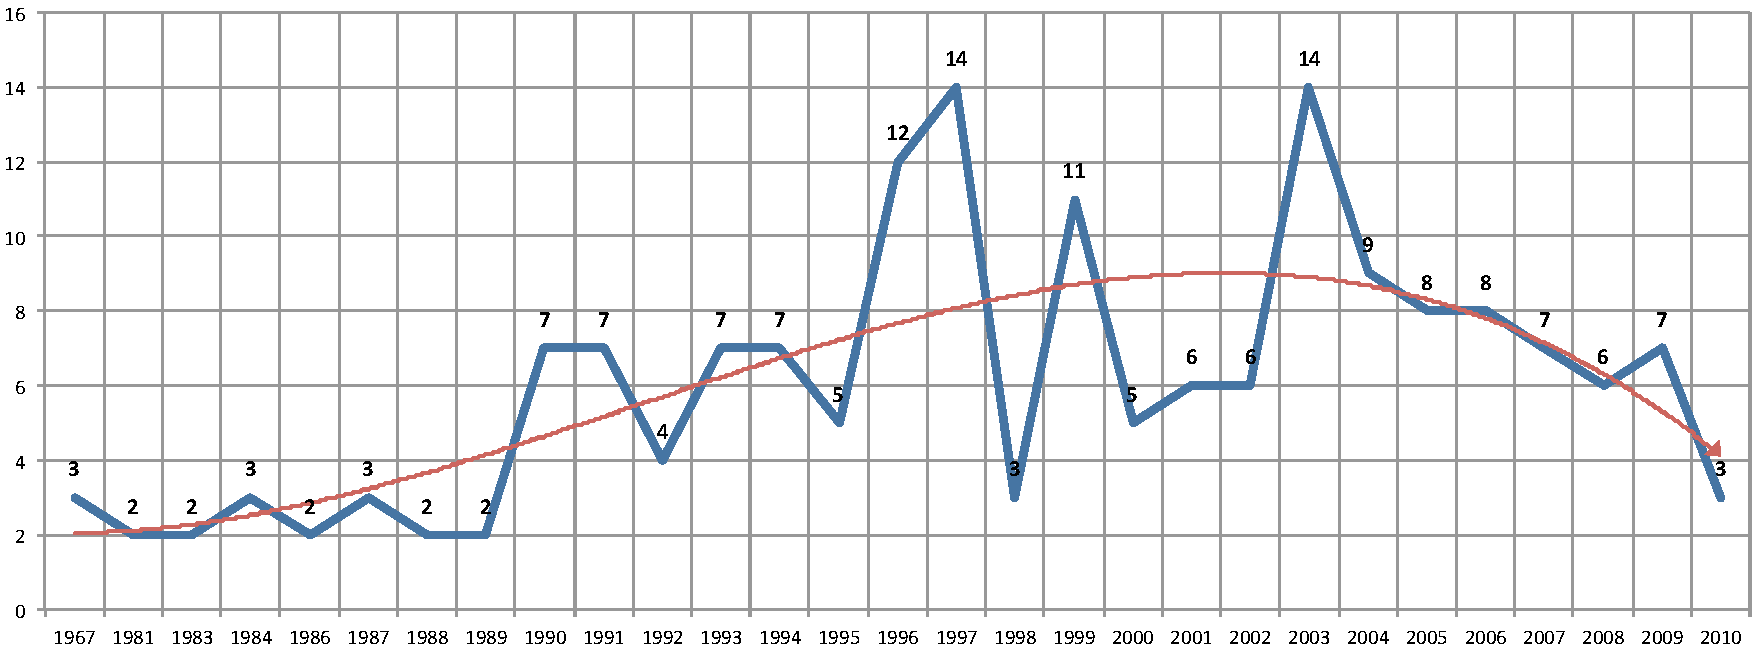
\includepdf[scale=0.5]{11-importedfigures/abntex2-modelo-img-grafico.pdf}
	\end{center}
	\legend{Fonte: \cite{araujo2012}}
\end{figure}

% ---
\subsection{Figuras em \emph{minipages}}
% ---

\emph{Minipages} são usadas para inserir textos ou outros elementos em quadros
com tamanhos e posições controladas. Veja o exemplo da
\autoref{fig_minipage_imagem1} e da \autoref{fig_minipage_grafico2}.

%\begin{figure}[htb]
% \label{teste}
% \centering
%  \begin{minipage}{0.4\textwidth}
%    \centering
%    \caption{Imagem 1 da minipage} \label{fig_minipage_imagem1}
%    
\includepdf[scale=0.9]{11-importedfigures/abntex2-modelo-img-marca.pdf}
%    \legend{Fonte: Produzido pelos autores}
%  \end{minipage}
%  \hfill
%  \begin{minipage}{0.4\textwidth}
%    \centering
%    \caption{Grafico 2 da minipage} \label{fig_minipage_grafico2}
%    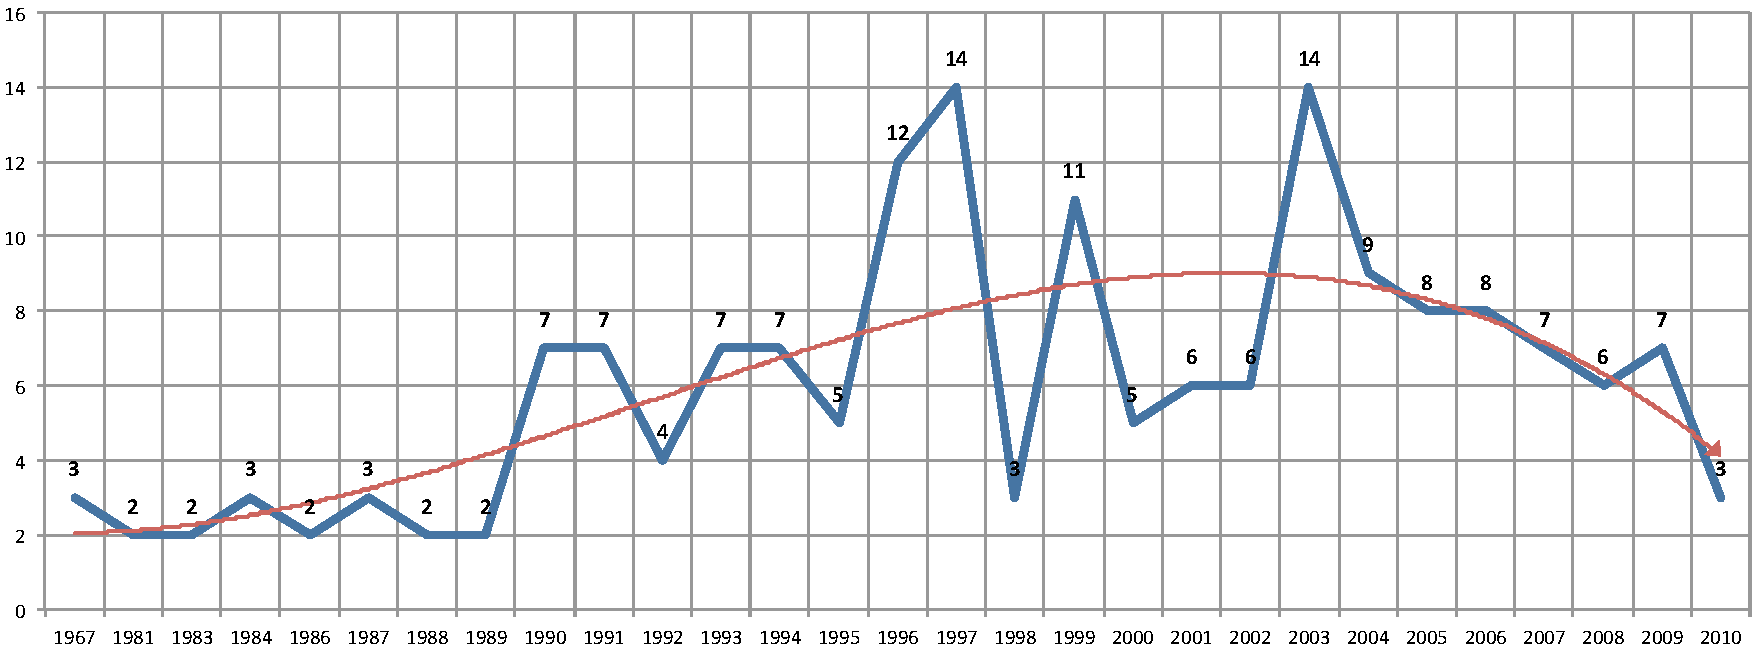
\includegraphics[scale=0.2]{11-importedfigures/abntex2-modelo-img-grafico.pdf}
%    \legend{Fonte: \cite{araujo2012}}
%  \end{minipage}
%\end{figure}

Observe que, segundo a \cite{NBR14724:2011}, as
ilustrações devem sempre ter numeração contínua e única em todo o documento:

\begin{citacao}
Qualquer que seja o tipo de ilustração, sua identificação aparece na parte
superior, precedida da palavra designativa (desenho, esquema, fluxograma,
fotografia, gráfico, mapa, organograma, planta, quadro, retrato, figura,
imagem, entre outros), seguida de seu número de ordem de ocorrência no texto,
em algarismos arábicos, travessão e do respectivo título. Após a ilustração, na
parte inferior, indicar a fonte consultada (elemento obrigatório, mesmo que
seja produção do próprio autor), legenda, notas e outras informações
necessárias à sua compreensão (se houver). A ilustração deve ser citada no
texto e inserida o mais próximo possível do trecho a que se
refere. \cite{NBR14724:2011}
\end{citacao}

% ---
\section{Expressões matemáticas}
% ---

\index{expressões matemáticas}Use o ambiente \texttt{equation} para escrever
expressões matemáticas numeradas:

\begin{equation}
  \forall x \in X, \quad \exists \: y \leq \epsilon
\end{equation}

Escreva expressões matemáticas entre \$ e \$, como em $ \lim_{x \to \infty}
\exp(-x) = 0 $, para que fiquem na mesma linha.

Também é possível usar colchetes para indicar o início de uma expressão
matemática que não é numerada.

\[
\left|\sum_{i=1}^n a_ib_i\right|
\le
\left(\sum_{i=1}^n a_i^2\right)^{1/2}
\left(\sum_{i=1}^n b_i^2\right)^{1/2}
\]

Consulte mais informações sobre expressões matemáticas em
\url{https://github.com/abntex/abntex2/wiki/Referencias}.

% ---
\section{Enumerações: alíneas e subalíneas}
% ---

\index{alíneas}\index{subalíneas}\index{incisos}Quando for necessário enumerar
os diversos assuntos de uma seção que não possua título, esta deve ser
subdividida em alíneas \cite{NBR6024:2012}:

\begin{alineas}

  \item os diversos assuntos que não possuam título próprio, dentro de uma mesma
  seção, devem ser subdivididos em alíneas; 
  
  \item o texto que antecede as alíneas termina em dois pontos;
  \item as alíneas devem ser indicadas alfabeticamente, em letra minúscula,
  seguida de parêntese. Utilizam-se letras dobradas, quando esgotadas as
  letras do alfabeto;

  \item as letras indicativas das alíneas devem apresentar recuo em relação à
  margem esquerda;

  \item o texto da alínea deve começar por letra minúscula e terminar em
  ponto-e-vírgula, exceto a última alínea que termina em ponto final;

  \item o texto da alínea deve terminar em dois pontos, se houver subalínea;

  \item a segunda e as seguintes linhas do texto da alínea começa sob a
  primeira letra do texto da própria alínea;
  
  \item subalíneas \cite{NBR6024:2012} devem ser conforme as alíneas a
  seguir:

  \begin{alineas}
     \item as subalíneas devem começar por travessão seguido de espaço;

     \item as subalíneas devem apresentar recuo em relação à alínea;

     \item o texto da subalínea deve começar por letra minúscula e terminar em
     ponto-e-vírgula. A última subalínea deve terminar em ponto final, se não
     houver alínea subsequente;

     \item a segunda e as seguintes linhas do texto da subalínea começam sob a
     primeira letra do texto da própria subalínea.
  \end{alineas}
  
  \item no \abnTeX\ estão disponíveis os ambientes \texttt{incisos} e
  \texttt{subalineas}, que em suma são o mesmo que se criar outro nível de
  \texttt{alineas}, como nos exemplos à seguir:
  
  \begin{incisos}
    \item \textit{Um novo inciso em itálico};
  \end{incisos}
  
  \item Alínea em \textbf{negrito}:
  
  \begin{subalineas}
    \item \textit{Uma subalínea em itálico};
    \item \underline{\textit{Uma subalínea em itálico e sublinhado}}; 
  \end{subalineas}
  
  \item Última alínea com \emph{ênfase}.
  
\end{alineas}

% ---
\section{Espaçamento entre parágrafos e linhas}
% ---

\index{espaçamento!dos parágrafos}O tamanho do parágrafo, espaço entre a margem
e o início da frase do parágrafo, é definido por:

\begin{verbatim}
   \setlength{\parindent}{1.3cm}
\end{verbatim}

\index{espaçamento!do primeiro parágrafo}Por padrão, não há espaçamento no
primeiro parágrafo de cada início de divisão do documento
(\autoref{sec-divisoes}). Porém, você pode definir que o primeiro parágrafo
também seja indentado, como é o caso deste documento. Para isso, apenas inclua o
pacote \textsf{indentfirst} no preâmbulo do documento:

\begin{verbatim}
   \usepackage{indentfirst}      % Indenta o primeiro parágrafo de cada seção.
\end{verbatim}

\index{espaçamento!entre os parágrafos}O espaçamento entre um parágrafo e outro
pode ser controlado por meio do comando:

\begin{verbatim}
  \setlength{\parskip}{0.2cm}  % tente também \onelineskip
\end{verbatim}

\index{espaçamento!entre as linhas}O controle do espaçamento entre linhas é
definido por:

\begin{verbatim}
  \OnehalfSpacing       % espaçamento um e meio (padrão); 
  \DoubleSpacing        % espaçamento duplo
  \SingleSpacing        % espaçamento simples	
\end{verbatim}

Para isso, também estão disponíveis os ambientes:

\begin{verbatim}
  \begin{SingleSpace} ...\end{SingleSpace}
  \begin{Spacing}{hfactori} ... \end{Spacing}
  \begin{OnehalfSpace} ... \end{OnehalfSpace}
  \begin{OnehalfSpace*} ... \end{OnehalfSpace*}
  \begin{DoubleSpace} ... \end{DoubleSpace}
  \begin{DoubleSpace*} ... \end{DoubleSpace*} 
\end{verbatim}

Para mais informações, consulte \cite{memoir}.

% ---
\section{Inclusão de outros arquivos}\label{sec-include}
% ---

É uma boa prática dividir o seu documento em diversos arquivos, e não
apenas escrever tudo em um único. Esse recurso foi utilizado neste
documento. Para incluir diferentes arquivos em um arquivo principal,
de modo que cada arquivo incluído fique em uma página diferente, utilize o
comando:

\begin{verbatim}
   \include{documento-a-ser-incluido}      % sem a extensão .tex
\end{verbatim}

Para incluir documentos sem quebra de páginas, utilize:

\begin{verbatim}
   \input{documento-a-ser-incluido}      % sem a extensão .tex
\end{verbatim}

% ---
\section{Compilar o documento \LaTeX}
% ---

Geralmente os editores \LaTeX, como o
TeXlipse\footnote{\url{http://texlipse.sourceforge.net/}}, o
Texmaker\footnote{\url{http://www.xm1math.net/texmaker/}}, entre outros,
compilam os documentos automaticamente, de modo que você não precisa se
preocupar com isso.

No entanto, você pode compilar os documentos \LaTeX usando os seguintes
comandos, que devem ser digitados no \emph{Prompt de Comandos} do Windows ou no
\emph{Terminal} do Mac ou do Linux:

\begin{verbatim}
   pdflatex ARQUIVO_PRINCIPAL.tex
   bibtex ARQUIVO_PRINCIPAL.aux
   makeindex ARQUIVO_PRINCIPAL.idx 
   makeindex ARQUIVO_PRINCIPAL.nlo -s nomencl.ist -o ARQUIVO_PRINCIPAL.nls
   pdflatex ARQUIVO_PRINCIPAL.tex
   pdflatex ARQUIVO_PRINCIPAL.tex
\end{verbatim}

% ---
\section{Remissões internas}
% ---

Ao nomear a \autoref{tab-nivinv} e a \autoref{fig_circulo}, apresentamos um
exemplo de remissão interna, que também pode ser feita quando indicamos o
\autoref{cap_exemplos}, que tem o nome \emph{\nameref{cap_exemplos}}. O número
do capítulo indicado é \ref{cap_exemplos}, que se inicia à
\autopageref{cap_exemplos}\footnote{O número da página de uma remissão pode ser
obtida também assim:
\pageref{cap_exemplos}.}.
Veja a \autoref{sec-divisoes} para outros exemplos de remissões internas entre
seções, subseções e subsubseções.

O código usado para produzir o texto desta seção é:

\begin{verbatim}
Ao nomear a \autoref{tab-nivinv} e a \autoref{fig_circulo}, apresentamos um
exemplo de remissão interna, que também pode ser feita quando indicamos o
\autoref{cap_exemplos}, que tem o nome \emph{\nameref{cap_exemplos}}. O número
do capítulo indicado é \ref{cap_exemplos}, que se inicia à
\autopageref{cap_exemplos}\footnote{O número da página de uma remissão pode ser
obtida também assim:
\pageref{cap_exemplos}.}.
Veja a \autoref{sec-divisoes} para outros exemplos de remissões internas entre
seções, subseções e subsubseções.
\end{verbatim}

% ---
\section{Divisões do documento: seção}\label{sec-divisoes}
% ---

Esta seção testa o uso de divisões de documentos. Esta é a
\autoref{sec-divisoes}. Veja a \autoref{sec-divisoes-subsection}.

\subsection{Divisões do documento: subseção}\label{sec-divisoes-subsection}

Isto é uma subseção. Veja a \autoref{sec-divisoes-subsubsection}, que é uma
\texttt{subsubsection} do \LaTeX, mas é impressa chamada de ``subseção'' porque
no Português não temos a palavra ``subsubseção''.

\subsubsection{Divisões do documento: subsubseção}
\label{sec-divisoes-subsubsection}

Isto é uma subsubseção.

\subsubsection{Divisões do documento: subsubseção}

Isto é outra subsubseção.

\subsection{Divisões do documento: subseção}\label{sec-exemplo-subsec}

Isto é uma subseção.

\subsubsection{Divisões do documento: subsubseção}

Isto é mais uma subsubseção da \autoref{sec-exemplo-subsec}.

%\subsubsubsection{Esta é uma subseção de quinto
%nível}\label{sec-exemplo-subsubsubsection}

%Esta é uma seção de quinto nível. Ela é produzida com o seguinte comando:

%\begin{verbatim}
%\subsubsubsection{Esta é uma subseção de quinto
%nível}\label{sec-exemplo-subsubsubsection}
%\end{verbatim}

%\subsubsubsection{Esta é outra subseção de quinto nível}\label{sec-exemplo-subsubsubsection-outro}

%Esta é outra seção de quinto nível.


%\paragraph{Este é um parágrafo numerado}\label{sec-exemplo-paragrafo}

ˆ%Este é um exemplo de parágrafo nomeado. Ele é produzida com o comando de
%parágrafo:

%\begin{verbatim}
%\paragraph{Este é um parágrafo nomeado}\label{sec-exemplo-paragrafo}
%\end{verbatim}

%A numeração entre parágrafos numeradaos e subsubsubseções são contínuas.

%\paragraph{Esta é outro parágrafo numerado}\label{sec-exemplo-paragrafo-outro}

%Esta é outro parágrafo nomeado.

% ---
%\section{Este é um exemplo de nome de seção longo. Ele deve estar
%alinhado à esquerda e a segunda e demais linhas devem iniciar logo abaixo da
%primeira palavra da primeira linha}
% ---

%Isso atende à norma \cite{NBR14724:2011} 
% e \cite{NBR6024:2012}.


% ---
\section{Diferentes idiomas e hifenizações}
\label{sec-hifenizacao}
% ---

Para usar hifenizações de diferentes idiomas, inclua nas opções do documento o
nome dos idiomas que o seu texto contém. Por exemplo (para melhor
visualização, as opções foram quebras em diferentes linhas):

\begin{verbatim}
\documentclass[
	12pt,
	openright,
	twoside,
	a4paper,
	english,
	french,
	spanish,
	brazil
	]{abntex2}
\end{verbatim}

O idioma português-brasileiro (\texttt{brazil}) é incluído automaticamente pela
classe \textsf{abntex2}. Porém, mesmo assim a opção \texttt{brazil} deve ser
informada como a última opção da classe para que todos os pacotes reconheçam o
idioma. Vale ressaltar que a última opção de idioma é a utilizada por padrão no
documento. Desse modo, caso deseje escrever um texto em inglês que tenha
citações em português e em francês, você deveria usar o preâmbulo como abaixo:

\begin{verbatim}
\documentclass[
	12pt,
	openright,
	twoside,
	a4paper,
	french,
	brazil,
	english
	]{abntex2}
\end{verbatim}

A lista completa de idiomas suportados, bem como outras opções de hifenização,
estão disponíveis em \cite{babel}.

Exemplo de hifenização em inglês\footnote{Extraído de:
\url{http://en.wikibooks.org/wiki/LaTeX/Internationalization}}:

\begin{otherlanguage*}{english}
\textit{Text in English language. This environment switches all language-related
definitions, like the language specific names for figures, tables etc. to the other
language. The starred version of this environment typesets the main text
according to the rules of the other language, but keeps the language specific
string for ancillary things like figures, in the main language of the document.
The environment hyphenrules switches only the hyphenation patterns used; it can
also be used to disallow hyphenation by using the language name
`nohyphenation'.}
\end{otherlanguage*}

Exemplo de hifenização em francês\footnote{Extraído de:
\url{http://bigbrowser.blog.lemonde.fr/2013/02/17/tu-ne-tweeteras-point-le-vatican-interdit-aux-cardinaux-de-tweeter-pendant-le-conclave/}}:

\begin{otherlanguage*}{french}
\textit{Texte en français. Pas question que Twitter ne vienne faire une
concurrence déloyale à la traditionnelle fumée blanche qui marque l'élection
d'un nouveau pape. Pour éviter toute fuite précoce, le Vatican a donc pris un
peu d'avance, et a déjà interdit aux cardinaux qui prendront part au vote
d'utiliser le réseau social, selon Catholic News Service. Une mesure valable
surtout pour les neuf cardinaux – sur les 117 du conclave – pratiquants très
actifs de Twitter, qui auront interdiction pendant toute la période de se
connecter à leur compte.}
\end{otherlanguage*}

Pequeno texto em espanhol\footnote{Extraído de:
\url{http://internacional.elpais.com/internacional/2013/02/17/actualidad/1361102009_913423.html}}:

\foreignlanguage{spanish}{\textit{Decenas de miles de personas ovacionan al pontífice en su
penúltimo ángelus dominical, el primero desde que anunciase su renuncia. El Papa se
centra en la crítica al materialismo}}.

O idioma geral do texto por ser alterado como no exemplo seguinte:

\begin{verbatim}
  \selectlanguage{english}
\end{verbatim}

Isso altera automaticamente a hifenização e todos os nomes constantes de
referências do documento para o idioma inglês. Consulte o manual da classe
\cite{abntex2classe} para obter orientações adicionais sobre internacionalização de
documentos produzidos com \abnTeX.

A \autoref{sec-citacao} descreve o ambiente \texttt{citacao} que pode receber
como parâmetro um idioma a ser usado na citação.

% ---
\section{Consulte o manual da classe \textsf{abntex2}}
% ---

Consulte o manual da classe \textsf{abntex2} \cite{abntex2classe} para uma
referência completa das macros e ambientes disponíveis. 

Além disso, o manual possui informações adicionais sobre as normas ABNT
observadas pelo \abnTeX\ e considerações sobre eventuais requisitos específicos
não atendidos, como o caso da \cite{NBR14724:2011}, que
especifica o espaçamento entre os capítulos e o início do texto, regra
propositalmente não atendida pelo presente modelo.

% ---
\section{Referências bibliográficas}
% ---

A formatação das referências bibliográficas conforme as regras da ABNT são um
dos principais objetivos do \abnTeX. Consulte os manuais
\cite{abntex2cite} e \cite{abntex2cite-alf} para obter informações
sobre como utilizar as referências bibliográficas.

%-
\subsection{Acentuação de referências bibliográficas}
%-

Normalmente não há problemas em usar caracteres acentuados em arquivos
bibliográficos (\texttt{*.bib}). Porém, como as regras da ABNT fazem uso quase
abusivo da conversão para letras maiúsculas, é preciso observar o modo como se
escreve os nomes dos autores. Na ~\autoref{tabela-acentos} você encontra alguns
exemplos das conversões mais importantes. Preste atenção especial para `ç' e `í'
que devem estar envoltos em chaves. A regra geral é sempre usar a acentuação
neste modo quando houver conversão para letras maiúsculas.

\begin{table}[htbp]
\caption{Tabela de conversão de acentuação.}
\label{tabela-acentos}

\begin{center}
\begin{tabular}{ll}\hline\hline
acento & \textsf{bibtex}\\
à á ã & \verb+\`a+ \verb+\'a+ \verb+\~a+\\
í & \verb+{\'\i}+\\
ç & \verb+{\c c}+\\
\hline\hline
\end{tabular}
\end{center}
\end{table}


% ---
\section{Precisa de ajuda?}
% ---

Consulte a FAQ com perguntas frequentes e comuns no portal do \abnTeX:
\url{https://github.com/abntex/abntex2/wiki/FAQ}.

Inscreva-se no grupo de usuários \LaTeX:
\url{http://groups.google.com/group/latex-br}, tire suas dúvidas e ajude
outros usuários.

Participe também do grupo de desenvolvedores do \abnTeX:
\url{http://groups.google.com/group/abntex2} e faça sua contribuição à
ferramenta.

% ---
\section{Você pode ajudar?}
% ---

Sua contribuição é muito importante! Você pode ajudar na divulgação, no
desenvolvimento e de várias outras formas. Veja como contribuir com o \abnTeX\
em \url{https://github.com/abntex/abntex2/wiki/Como-Contribuir}.

% ---
\section{Quer customizar os modelos do \abnTeX\ para sua instituição ou
universidade?}
% ---

Veja como customizar o \abnTeX\ em:
\url{https://github.com/abntex/abntex2/wiki/ComoCustomizar}.



\chapter{Conteúdos específicos do modelo de trabalho acadêmico}\label{cap_trabalho_academico}

\section{Quadros}

Este modelo vem com o ambiente \texttt{quadro} e impressão de Lista de quadros
configurados por padrão. Verifique um exemplo de utilização:

\begin{quadro}[htb]
\caption{\label{quadro_exemplo}Exemplo de quadro}
\begin{tabular}{|c|c|c|c|}
	\hline
	\textbf{Pessoa} & \textbf{Idade} & \textbf{Peso} & \textbf{Altura} \\ \hline
	Marcos & 26    & 68   & 178    \\ \hline
	Ivone  & 22    & 57   & 162    \\ \hline
	...    & ...   & ...  & ...    \\ \hline
	Sueli  & 40    & 65   & 153    \\ \hline
\end{tabular}
\fonte{Autor.}
\end{quadro}

Este parágrafo apresenta como referenciar o quadro no texto, requisito
obrigatório da ABNT.
Primeira opção, utilizando \texttt{autoref}: Ver o \autoref{quadro_exemplo}.
Segunda opção, utilizando \texttt{ref}: Ver o Quadro \ref{quadro_exemplo}.

\part{Resultados}

\chapter{Dados e Análises com Códigos R}

Abaixo é um teste para geração de Tabelas com código R dentro do environment Latex

\begin{tabular}{l|l}
\hline
Simbolo & Descrição\\
\hline
A & Descrição A\\
\hline
B & Descrição B\\
\hline
C & Descrição C\\
\hline
\end{tabular}

Calculando a média no R:

\begin{Shaded}
\begin{Highlighting}[]
\NormalTok{vector <-}\StringTok{ }\KeywordTok{c}\NormalTok{(}\DecValTok{2}\NormalTok{,}\DecValTok{4}\NormalTok{,}\DecValTok{6}\NormalTok{,}\DecValTok{8}\NormalTok{,}\DecValTok{10}\NormalTok{)}
\NormalTok{mean.vector <-}\StringTok{ }\KeywordTok{mean}\NormalTok{(vector)}
\KeywordTok{cat}\NormalTok{(}\StringTok{'A média do vetor é:'}\NormalTok{, mean.vector)}
\end{Highlighting}
\end{Shaded}

A média do vetor é: 6

\begin{Shaded}
\begin{Highlighting}[]
\KeywordTok{summary}\NormalTok{(mtcars)}
\end{Highlighting}
\end{Shaded}

\begin{verbatim}
  mpg             cyl             disp             hp       
\end{verbatim}

Min. :10.40 Min. :4.000 Min. : 71.1 Min. : 52.0\\
1st Qu.:15.43 1st Qu.:4.000 1st Qu.:120.8 1st Qu.: 96.5\\
Median :19.20 Median :6.000 Median :196.3 Median :123.0\\
Mean :20.09 Mean :6.188 Mean :230.7 Mean :146.7\\
3rd Qu.:22.80 3rd Qu.:8.000 3rd Qu.:326.0 3rd Qu.:180.0\\
Max. :33.90 Max. :8.000 Max. :472.0 Max. :335.0\\
drat wt qsec vs\\
Min. :2.760 Min. :1.513 Min. :14.50 Min. :0.0000\\
1st Qu.:3.080 1st Qu.:2.581 1st Qu.:16.89 1st Qu.:0.0000\\
Median :3.695 Median :3.325 Median :17.71 Median :0.0000\\
Mean :3.597 Mean :3.217 Mean :17.85 Mean :0.4375\\
3rd Qu.:3.920 3rd Qu.:3.610 3rd Qu.:18.90 3rd Qu.:1.0000\\
Max. :4.930 Max. :5.424 Max. :22.90 Max. :1.0000\\
am gear carb\\
Min. :0.0000 Min. :3.000 Min. :1.000\\
1st Qu.:0.0000 1st Qu.:3.000 1st Qu.:2.000\\
Median :0.0000 Median :4.000 Median :2.000\\
Mean :0.4062 Mean :3.688 Mean :2.812\\
3rd Qu.:1.0000 3rd Qu.:4.000 3rd Qu.:4.000\\
Max. :1.0000 Max. :5.000 Max. :8.000

\begin{Shaded}
\begin{Highlighting}[]
\KeywordTok{str}\NormalTok{(mtcars)}
\end{Highlighting}
\end{Shaded}

`data.frame': 32 obs. of 11 variables:
\$ mpg : num 21 21 22.8 21.4 18.7 18.1 14.3 24.4 22.8 19.2 \ldots{}
\$ cyl : num 6 6 4 6 8 6 8 4 4 6 \ldots{}
\$ disp: num 160 160 108 258 360 \ldots{}
\$ hp : num 110 110 93 110 175 105 245 62 95 123 \ldots{}
\$ drat: num 3.9 3.9 3.85 3.08 3.15 2.76 3.21 3.69 3.92 3.92 \ldots{}
\$ wt : num 2.62 2.88 2.32 3.21 3.44 \ldots{}
\$ qsec: num 16.5 17 18.6 19.4 17 \ldots{}
\$ vs : num 0 0 1 1 0 1 0 1 1 1 \ldots{}
\$ am : num 1 1 1 0 0 0 0 0 0 0 \ldots{}
\$ gear: num 4 4 4 3 3 3 3 4 4 4 \ldots{}
\$ carb: num 4 4 1 1 2 1 4 2 2 4 \ldots{}

Modelo de gráfico em código R:

\begin{center}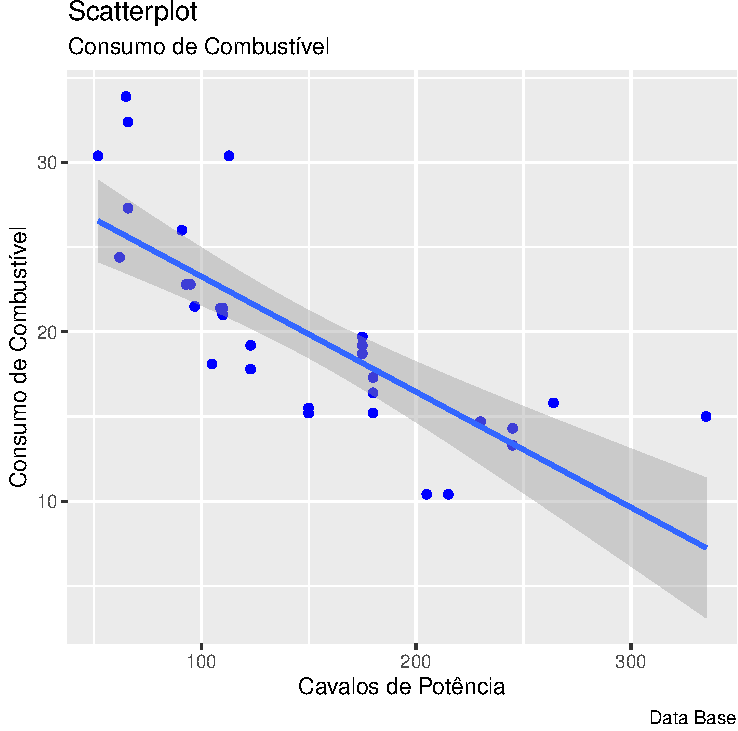
\includegraphics{thesis_files/figure-latex/unnamed-chunk-6-1} \end{center}
\begin{figure}[!htb]
\centering
\caption{Gráfico GGPlot para Teste}
\label{fig:ggplot}
\end{figure}

\section{Regressão com Código R}

Seguem abaixo exemplos\footnote{Os exemplos demonstrados são reproduções de partes do curso de Regressão Linear da Universidade Johns Hopkins} de inserção de códigos R para captura, tratamento, exploração, análises econométrica, predições, construção de algorítimos e formulas.

\hypertarget{swiss-fertility-data}{%
\subsection{Swiss fertility data}\label{swiss-fertility-data}}

\begin{Shaded}
\begin{Highlighting}[]
\KeywordTok{library}\NormalTok{(datasets); }\KeywordTok{data}\NormalTok{(swiss); }\KeywordTok{require}\NormalTok{(stats); }\KeywordTok{require}\NormalTok{(graphics)}
\KeywordTok{pairs}\NormalTok{(swiss, }\DataTypeTok{panel =}\NormalTok{ panel.smooth, }\DataTypeTok{main =} \StringTok{"Swiss data"}\NormalTok{, }\DataTypeTok{col =} \DecValTok{3} \OperatorTok{+}\StringTok{ }\NormalTok{(swiss}\OperatorTok{$}\NormalTok{Catholic }\OperatorTok{>}\StringTok{ }\DecValTok{50}\NormalTok{))}
\end{Highlighting}
\end{Shaded}

\hypertarget{swiss}{%
\subsection{\texorpdfstring{\texttt{?swiss}}{?swiss}}\label{swiss}}

\hypertarget{description}{%
\subsubsection{Description}\label{description}}

Standardized fertility measure and socio-economic indicators for each of 47 French-speaking provinces of Switzerland at about 1888.

A data frame with 47 observations on 6 variables, each of which is in percent, i.e., in {[}0, 100{]}.

\begin{itemize}
\tightlist
\item
  {[},1{]} Fertility Ig, ` common standardized fertility measure'
\item
  {[},2{]} Agriculture \% of males involved in agriculture as occupation
\item
  {[},3{]} Examination \% draftees receiving highest mark on army examination
\item
  {[},4{]} Education \% education beyond primary school for draftees.
\item
  {[},5{]} Catholic \% `catholic' (as opposed to `protestant').
\item
  {[},6{]} Infant.Mortality live births who live less than 1 year.
\end{itemize}

All variables but `Fertility' give proportions of the population.

\hypertarget{calling-lm}{%
\subsection{\texorpdfstring{Calling \texttt{lm}}{Calling lm}}\label{calling-lm}}

\texttt{summary(lm(Fertility\ \textasciitilde{}\ .\ ,\ data\ =\ swiss))}

\begin{verbatim}
                   Estimate  Std. Error   t value     Pr(>|t|)
(Intercept)      66.9151817 10.70603759  6.250229 1.906051e-07
Agriculture      -0.1721140  0.07030392 -2.448142 1.872715e-02
Examination      -0.2580082  0.25387820 -1.016268 3.154617e-01
Education        -0.8709401  0.18302860 -4.758492 2.430605e-05
Catholic          0.1041153  0.03525785  2.952969 5.190079e-03
Infant.Mortality  1.0770481  0.38171965  2.821568 7.335715e-03
\end{verbatim}

\hypertarget{example-interpretation}{%
\subsection{Example interpretation}\label{example-interpretation}}

\begin{itemize}
\tightlist
\item
  Agriculture is expressed in percentages (0 - 100)
\item
  Estimate is -0.1721.
\item
  We estimate an expected 0.17 decrease in standardized fertility for every 1\% increase in percentage of males involved in agriculture in holding the remaining variables constant.
\item
  The t-test for \(H_0: \beta_{Agri} = 0\) versus \(H_a: \beta_{Agri} \neq 0\) is significant.
\item
  Interestingly, the unadjusted estimate is
\end{itemize}

\begin{Shaded}
\begin{Highlighting}[]
\KeywordTok{summary}\NormalTok{(}\KeywordTok{lm}\NormalTok{(Fertility }\OperatorTok{~}\StringTok{ }\NormalTok{Agriculture, }\DataTypeTok{data =}\NormalTok{ swiss))}\OperatorTok{$}\NormalTok{coefficients}
\end{Highlighting}
\end{Shaded}

\begin{verbatim}
              Estimate Std. Error   t value     Pr(>|t|)
(Intercept) 60.3043752 4.25125562 14.185074 3.216304e-18
Agriculture  0.1942017 0.07671176  2.531577 1.491720e-02
\end{verbatim}

How can adjustment reverse the sign of an effect? Let's try a simulation.

\begin{Shaded}
\begin{Highlighting}[]
\NormalTok{n <-}\StringTok{ }\DecValTok{100}\NormalTok{; x2 <-}\StringTok{ }\DecValTok{1} \OperatorTok{:}\StringTok{ }\NormalTok{n; x1 <-}\StringTok{ }\FloatTok{.01} \OperatorTok{*}\StringTok{ }\NormalTok{x2 }\OperatorTok{+}\StringTok{ }\KeywordTok{runif}\NormalTok{(n, }\FloatTok{-.1}\NormalTok{, }\FloatTok{.1}\NormalTok{); y =}\StringTok{ }\OperatorTok{-}\NormalTok{x1 }\OperatorTok{+}\StringTok{ }\NormalTok{x2 }\OperatorTok{+}\StringTok{ }\KeywordTok{rnorm}\NormalTok{(n, }\DataTypeTok{sd =} \FloatTok{.01}\NormalTok{)}
\KeywordTok{summary}\NormalTok{(}\KeywordTok{lm}\NormalTok{(y }\OperatorTok{~}\StringTok{ }\NormalTok{x1))}\OperatorTok{$}\NormalTok{coef}
\end{Highlighting}
\end{Shaded}

\begin{verbatim}
              Estimate Std. Error    t value     Pr(>|t|)
(Intercept)  0.4501325   1.196004  0.3763638 7.074600e-01
x1          98.1991010   2.064007 47.5769327 1.575874e-69
\end{verbatim}

\begin{Shaded}
\begin{Highlighting}[]
\KeywordTok{summary}\NormalTok{(}\KeywordTok{lm}\NormalTok{(y }\OperatorTok{~}\StringTok{ }\NormalTok{x1 }\OperatorTok{+}\StringTok{ }\NormalTok{x2))}\OperatorTok{$}\NormalTok{coef}
\end{Highlighting}
\end{Shaded}

\begin{verbatim}
                 Estimate   Std. Error      t value      Pr(>|t|)
(Intercept) -0.0009920596 0.0020522991   -0.4833894  6.299087e-01
x1          -0.9957394976 0.0175425669  -56.7613340  3.193593e-76
x2           0.9999446100 0.0001732035 5773.2359436 2.559355e-270
\end{verbatim}

\hypertarget{back-to-this-data-set}{%
\subsection{Back to this data set}\label{back-to-this-data-set}}

\begin{itemize}
\tightlist
\item
  The sign reverses itself with the inclusion of Examination and Education, but of which are negatively correlated with Agriculture.
\item
  The percent of males in the province working in agriculture is negatively related to educational attainment (correlation of -0.6395225) and Education and Examination (correlation of 0.6984153) are obviously measuring similar things.

  \begin{itemize}
  \tightlist
  \item
    Is the positive marginal an artifact for not having accounted for, say, Education level? (Education does have a stronger effect, by the way.)
  \end{itemize}
\item
  At the minimum, anyone claiming that provinces that are more agricultural have higher fertility rates would immediately be open to criticism.
\end{itemize}

\hypertarget{what-if-we-include-an-unnecessary-variable}{%
\subsection{What if we include an unnecessary variable?}\label{what-if-we-include-an-unnecessary-variable}}

z adds no new linear information, since it's a linear
combination of variables already included. R just drops
terms that are linear combinations of other terms.

\begin{Shaded}
\begin{Highlighting}[]
\NormalTok{z <-}\StringTok{ }\NormalTok{swiss}\OperatorTok{$}\NormalTok{Agriculture }\OperatorTok{+}\StringTok{ }\NormalTok{swiss}\OperatorTok{$}\NormalTok{Education}
\KeywordTok{lm}\NormalTok{(Fertility }\OperatorTok{~}\StringTok{ }\NormalTok{. }\OperatorTok{+}\StringTok{ }\NormalTok{z, }\DataTypeTok{data =}\NormalTok{ swiss)}
\end{Highlighting}
\end{Shaded}

\begin{verbatim}

Call:
lm(formula = Fertility ~ . + z, data = swiss)

Coefficients:
     (Intercept)       Agriculture       Examination         Education          Catholic  
         66.9152           -0.1721           -0.2580           -0.8709            0.1041  
Infant.Mortality                 z  
          1.0770                NA  
\end{verbatim}

\hypertarget{dummy-variables-are-smart}{%
\subsection{Dummy variables are smart}\label{dummy-variables-are-smart}}

\begin{itemize}
\tightlist
\item
  Consider the linear model
  \[
  Y_i = \beta_0 + X_{i1} \beta_1 + \epsilon_{i}
  \]
  where each \(X_{i1}\) is binary so that it is a 1 if measurement \(i\) is in a group and 0 otherwise. (Treated versus not in a clinical trial, for example.)
\item
  Then for people in the group \(E[Y_i] = \beta_0 + \beta_1\)
\item
  And for people not in the group \(E[Y_i] = \beta_0\)
\item
  The LS fits work out to be \(\hat \beta_0 + \hat \beta_1\) is the mean for those in the group and \(\hat \beta_0\) is the mean for those not in the group.
\item
  \(\beta_1\) is interpretted as the increase or decrease in the mean comparing those in the group to those not.
\item
  Note including a binary variable that is 1 for those not in the group would be redundant. It would create three parameters to describe two means.
\end{itemize}

\hypertarget{more-than-2-levels}{%
\subsection{More than 2 levels}\label{more-than-2-levels}}

\begin{itemize}
\tightlist
\item
  Consider a multilevel factor level. For didactic reasons, let's say a three level factor (example, US political party affiliation: Republican, Democrat, Independent)
\item
  \(Y_i = \beta_0 + X_{i1} \beta_1 + X_{i2} \beta_2 + \epsilon_i\).
\item
  \(X_{i1}\) is 1 for Republicans and 0 otherwise.
\item
  \(X_{i2}\) is 1 for Democrats and 0 otherwise.
\item
  If \(i\) is Republican \(E[Y_i] = \beta_0 +\beta_1\)
\item
  If \(i\) is Democrat \(E[Y_i] = \beta_0 + \beta_2\).
\item
  If \(i\) is Independent \(E[Y_i] = \beta_0\).
\item
  \(\beta_1\) compares Republicans to Independents.
\item
  \(\beta_2\) compares Democrats to Independents.
\item
  \(\beta_1 - \beta_2\) compares Republicans to Democrats.
\item
  (Choice of reference category changes the interpretation.)
\end{itemize}

\hypertarget{insect-sprays}{%
\subsection{Insect Sprays}\label{insect-sprays}}

\hypertarget{linear-model-fit-group-a-is-the-reference}{%
\subsection{Linear model fit, group A is the reference}\label{linear-model-fit-group-a-is-the-reference}}

\begin{Shaded}
\begin{Highlighting}[]
\KeywordTok{summary}\NormalTok{(}\KeywordTok{lm}\NormalTok{(count }\OperatorTok{~}\StringTok{ }\NormalTok{spray, }\DataTypeTok{data =}\NormalTok{ InsectSprays))}\OperatorTok{$}\NormalTok{coef}
\end{Highlighting}
\end{Shaded}

\begin{verbatim}
               Estimate Std. Error    t value     Pr(>|t|)
(Intercept)  14.5000000   1.132156 12.8074279 1.470512e-19
sprayB        0.8333333   1.601110  0.5204724 6.044761e-01
sprayC      -12.4166667   1.601110 -7.7550382 7.266893e-11
sprayD       -9.5833333   1.601110 -5.9854322 9.816910e-08
sprayE      -11.0000000   1.601110 -6.8702352 2.753922e-09
sprayF        2.1666667   1.601110  1.3532281 1.805998e-01
\end{verbatim}

\hypertarget{hard-coding-the-dummy-variables}{%
\subsection{Hard coding the dummy variables}\label{hard-coding-the-dummy-variables}}

\begin{Shaded}
\begin{Highlighting}[]
\KeywordTok{summary}\NormalTok{(}\KeywordTok{lm}\NormalTok{(count }\OperatorTok{~}\StringTok{ }
\StringTok{             }\KeywordTok{I}\NormalTok{(}\DecValTok{1} \OperatorTok{*}\StringTok{ }\NormalTok{(spray }\OperatorTok{==}\StringTok{ 'B'}\NormalTok{)) }\OperatorTok{+}\StringTok{ }\KeywordTok{I}\NormalTok{(}\DecValTok{1} \OperatorTok{*}\StringTok{ }\NormalTok{(spray }\OperatorTok{==}\StringTok{ 'C'}\NormalTok{)) }\OperatorTok{+}\StringTok{ }
\StringTok{             }\KeywordTok{I}\NormalTok{(}\DecValTok{1} \OperatorTok{*}\StringTok{ }\NormalTok{(spray }\OperatorTok{==}\StringTok{ 'D'}\NormalTok{)) }\OperatorTok{+}\StringTok{ }\KeywordTok{I}\NormalTok{(}\DecValTok{1} \OperatorTok{*}\StringTok{ }\NormalTok{(spray }\OperatorTok{==}\StringTok{ 'E'}\NormalTok{)) }\OperatorTok{+}
\StringTok{             }\KeywordTok{I}\NormalTok{(}\DecValTok{1} \OperatorTok{*}\StringTok{ }\NormalTok{(spray }\OperatorTok{==}\StringTok{ 'F'}\NormalTok{))}
\NormalTok{           , }\DataTypeTok{data =}\NormalTok{ InsectSprays))}\OperatorTok{$}\NormalTok{coef}
\end{Highlighting}
\end{Shaded}

\begin{verbatim}
                         Estimate Std. Error    t value     Pr(>|t|)
(Intercept)            14.5000000   1.132156 12.8074279 1.470512e-19
I(1 * (spray == "B"))   0.8333333   1.601110  0.5204724 6.044761e-01
I(1 * (spray == "C")) -12.4166667   1.601110 -7.7550382 7.266893e-11
I(1 * (spray == "D"))  -9.5833333   1.601110 -5.9854322 9.816910e-08
I(1 * (spray == "E")) -11.0000000   1.601110 -6.8702352 2.753922e-09
I(1 * (spray == "F"))   2.1666667   1.601110  1.3532281 1.805998e-01
\end{verbatim}

\hypertarget{what-if-we-include-all-6}{%
\subsection{What if we include all 6?}\label{what-if-we-include-all-6}}

\begin{Shaded}
\begin{Highlighting}[]
\KeywordTok{lm}\NormalTok{(count }\OperatorTok{~}\StringTok{ }
\StringTok{   }\KeywordTok{I}\NormalTok{(}\DecValTok{1} \OperatorTok{*}\StringTok{ }\NormalTok{(spray }\OperatorTok{==}\StringTok{ 'B'}\NormalTok{)) }\OperatorTok{+}\StringTok{ }\KeywordTok{I}\NormalTok{(}\DecValTok{1} \OperatorTok{*}\StringTok{ }\NormalTok{(spray }\OperatorTok{==}\StringTok{ 'C'}\NormalTok{)) }\OperatorTok{+}\StringTok{  }
\StringTok{   }\KeywordTok{I}\NormalTok{(}\DecValTok{1} \OperatorTok{*}\StringTok{ }\NormalTok{(spray }\OperatorTok{==}\StringTok{ 'D'}\NormalTok{)) }\OperatorTok{+}\StringTok{ }\KeywordTok{I}\NormalTok{(}\DecValTok{1} \OperatorTok{*}\StringTok{ }\NormalTok{(spray }\OperatorTok{==}\StringTok{ 'E'}\NormalTok{)) }\OperatorTok{+}
\StringTok{   }\KeywordTok{I}\NormalTok{(}\DecValTok{1} \OperatorTok{*}\StringTok{ }\NormalTok{(spray }\OperatorTok{==}\StringTok{ 'F'}\NormalTok{)) }\OperatorTok{+}\StringTok{ }\KeywordTok{I}\NormalTok{(}\DecValTok{1} \OperatorTok{*}\StringTok{ }\NormalTok{(spray }\OperatorTok{==}\StringTok{ 'A'}\NormalTok{)), }\DataTypeTok{data =}\NormalTok{ InsectSprays)}
\end{Highlighting}
\end{Shaded}

\begin{verbatim}

Call:
lm(formula = count ~ I(1 * (spray == "B")) + I(1 * (spray == 
    "C")) + I(1 * (spray == "D")) + I(1 * (spray == "E")) + I(1 * 
    (spray == "F")) + I(1 * (spray == "A")), data = InsectSprays)

Coefficients:
          (Intercept)  I(1 * (spray == "B"))  I(1 * (spray == "C"))  I(1 * (spray == "D"))  
              14.5000                 0.8333               -12.4167                -9.5833  
I(1 * (spray == "E"))  I(1 * (spray == "F"))  I(1 * (spray == "A"))  
             -11.0000                 2.1667                     NA  
\end{verbatim}

\hypertarget{what-if-we-omit-the-intercept}{%
\subsection{What if we omit the intercept?}\label{what-if-we-omit-the-intercept}}

\begin{Shaded}
\begin{Highlighting}[]
\KeywordTok{summary}\NormalTok{(}\KeywordTok{lm}\NormalTok{(count }\OperatorTok{~}\StringTok{ }\NormalTok{spray }\OperatorTok{-}\StringTok{ }\DecValTok{1}\NormalTok{, }\DataTypeTok{data =}\NormalTok{ InsectSprays))}\OperatorTok{$}\NormalTok{coef}
\end{Highlighting}
\end{Shaded}

\begin{verbatim}
        Estimate Std. Error   t value     Pr(>|t|)
sprayA 14.500000   1.132156 12.807428 1.470512e-19
sprayB 15.333333   1.132156 13.543487 1.001994e-20
sprayC  2.083333   1.132156  1.840148 7.024334e-02
sprayD  4.916667   1.132156  4.342749 4.953047e-05
sprayE  3.500000   1.132156  3.091448 2.916794e-03
sprayF 16.666667   1.132156 14.721181 1.573471e-22
\end{verbatim}

\begin{Shaded}
\begin{Highlighting}[]
\KeywordTok{unique}\NormalTok{(}\KeywordTok{ave}\NormalTok{(InsectSprays}\OperatorTok{$}\NormalTok{count, InsectSprays}\OperatorTok{$}\NormalTok{spray))}
\end{Highlighting}
\end{Shaded}

\begin{verbatim}
[1] 14.500000 15.333333  2.083333  4.916667  3.500000 16.666667
\end{verbatim}

\hypertarget{summary}{%
\subsection{Summary}\label{summary}}

\begin{itemize}
\tightlist
\item
  If we treat Spray as a factor, R includes an intercept and omits the alphabetically first level of the factor.

  \begin{itemize}
  \tightlist
  \item
    All t-tests are for comparisons of Sprays versus Spray A.
  \item
    Emprirical mean for A is the intercept.
  \item
    Other group means are the itc plus their coefficient.
  \end{itemize}
\item
  If we omit an intercept, then it includes terms for all levels of the factor.

  \begin{itemize}
  \tightlist
  \item
    Group means are the coefficients.
  \item
    Tests are tests of whether the groups are different than zero. (Are the expected counts zero for that spray.)
  \end{itemize}
\item
  If we want comparisons between, Spray B and C, say we could refit the model with C (or B) as the reference level.
\end{itemize}

Reordering the levels

\begin{Shaded}
\begin{Highlighting}[]
\NormalTok{spray2 <-}\StringTok{ }\KeywordTok{relevel}\NormalTok{(InsectSprays}\OperatorTok{$}\NormalTok{spray, }\StringTok{"C"}\NormalTok{)}
\KeywordTok{summary}\NormalTok{(}\KeywordTok{lm}\NormalTok{(count }\OperatorTok{~}\StringTok{ }\NormalTok{spray2, }\DataTypeTok{data =}\NormalTok{ InsectSprays))}\OperatorTok{$}\NormalTok{coef}
\end{Highlighting}
\end{Shaded}

\begin{verbatim}
             Estimate Std. Error  t value     Pr(>|t|)
(Intercept)  2.083333   1.132156 1.840148 7.024334e-02
spray2A     12.416667   1.601110 7.755038 7.266893e-11
spray2B     13.250000   1.601110 8.275511 8.509776e-12
spray2D      2.833333   1.601110 1.769606 8.141205e-02
spray2E      1.416667   1.601110 0.884803 3.794750e-01
spray2F     14.583333   1.601110 9.108266 2.794343e-13
\end{verbatim}

Doing it manually
Equivalently
\[Var(\hat \beta_B - \hat \beta_C) = Var(\hat \beta_B) + Var(\hat \beta_C) - 2 Cov(\hat \beta_B, \hat \beta_C)\]

\begin{Shaded}
\begin{Highlighting}[]
\NormalTok{fit <-}\StringTok{ }\KeywordTok{lm}\NormalTok{(count }\OperatorTok{~}\StringTok{ }\NormalTok{spray, }\DataTypeTok{data =}\NormalTok{ InsectSprays) }\CommentTok{#A is ref}
\NormalTok{bbmbc <-}\StringTok{ }\KeywordTok{coef}\NormalTok{(fit)[}\DecValTok{2}\NormalTok{] }\OperatorTok{-}\StringTok{ }\KeywordTok{coef}\NormalTok{(fit)[}\DecValTok{3}\NormalTok{] }\CommentTok{#B - C}
\NormalTok{temp <-}\StringTok{ }\KeywordTok{summary}\NormalTok{(fit) }
\NormalTok{se <-}\StringTok{ }\NormalTok{temp}\OperatorTok{$}\NormalTok{sigma }\OperatorTok{*}\StringTok{ }\KeywordTok{sqrt}\NormalTok{(temp}\OperatorTok{$}\NormalTok{cov.unscaled[}\DecValTok{2}\NormalTok{, }\DecValTok{2}\NormalTok{] }\OperatorTok{+}\StringTok{ }\NormalTok{temp}\OperatorTok{$}\NormalTok{cov.unscaled[}\DecValTok{3}\NormalTok{,}\DecValTok{3}\NormalTok{] }\OperatorTok{-}\StringTok{ }\DecValTok{2} \OperatorTok{*}\NormalTok{temp}\OperatorTok{$}\NormalTok{cov.unscaled[}\DecValTok{2}\NormalTok{,}\DecValTok{3}\NormalTok{])}
\NormalTok{t <-}\StringTok{ }\NormalTok{(bbmbc) }\OperatorTok{/}\StringTok{ }\NormalTok{se}
\NormalTok{p <-}\StringTok{ }\KeywordTok{pt}\NormalTok{(}\OperatorTok{-}\KeywordTok{abs}\NormalTok{(t), }\DataTypeTok{df =}\NormalTok{ fit}\OperatorTok{$}\NormalTok{df)}
\NormalTok{out <-}\StringTok{ }\KeywordTok{c}\NormalTok{(bbmbc, se, t, p)}
\KeywordTok{names}\NormalTok{(out) <-}\StringTok{ }\KeywordTok{c}\NormalTok{(}\StringTok{"B - C"}\NormalTok{, }\StringTok{"SE"}\NormalTok{, }\StringTok{"T"}\NormalTok{, }\StringTok{"P"}\NormalTok{)}
\KeywordTok{round}\NormalTok{(out, }\DecValTok{3}\NormalTok{)}
\end{Highlighting}
\end{Shaded}

\begin{verbatim}
 B - C     SE      T      P 
13.250  1.601  8.276  0.000 
\end{verbatim}

\hypertarget{other-thoughts-on-this-data}{%
\subsection{Other thoughts on this data}\label{other-thoughts-on-this-data}}

\begin{itemize}
\tightlist
\item
  Counts are bounded from below by 0, violates the assumption of normality of the errors.

  \begin{itemize}
  \tightlist
  \item
    Also there are counts near zero, so both the actual assumption and the intent of the assumption are violated.
  \end{itemize}
\item
  Variance does not appear to be constant.
\item
  Perhaps taking logs of the counts would help.

  \begin{itemize}
  \tightlist
  \item
    There are 0 counts, so maybe log(Count + 1)
  \end{itemize}
\item
  Also, we'll cover Poisson GLMs for fitting count data.
\end{itemize}

WHO childhood hunger data

\begin{Shaded}
\begin{Highlighting}[]
\CommentTok{#download.file("http://apps.who.int/gho/athena/data/GHO/WHOSIS_000008.csv?profile=text&filter=COUNTRY:*;SEX:*","hunger.csv",method="curl")}
\NormalTok{hunger <-}\StringTok{ }\KeywordTok{read.csv}\NormalTok{(}\StringTok{'01-data/sheets/hunger.csv'}\NormalTok{)}
\NormalTok{hunger <-}\StringTok{ }\NormalTok{hunger[hunger}\OperatorTok{$}\NormalTok{Sex}\OperatorTok{!=}\StringTok{"Both sexes"}\NormalTok{,]}
\KeywordTok{head}\NormalTok{(hunger)}
\end{Highlighting}
\end{Shaded}

\begin{verbatim}
                               Indicator Data.Source PUBLISH.STATES Year            WHO.region
1 Children aged <5 years underweight (%) NLIS_310044      Published 1986                Africa
2 Children aged <5 years underweight (%) NLIS_310233      Published 1990              Americas
3 Children aged <5 years underweight (%) NLIS_312902      Published 2005              Americas
5 Children aged <5 years underweight (%) NLIS_312522      Published 2002 Eastern Mediterranean
6 Children aged <5 years underweight (%) NLIS_312955      Published 2008                Africa
8 Children aged <5 years underweight (%) NLIS_312963      Published 2008                Africa
        Country    Sex Display.Value Numeric Low High Comments
1       Senegal   Male          19.3    19.3  NA   NA       NA
2      Paraguay   Male           2.2     2.2  NA   NA       NA
3     Nicaragua   Male           5.3     5.3  NA   NA       NA
5        Jordan Female           3.2     3.2  NA   NA       NA
6 Guinea-Bissau Female          17.0    17.0  NA   NA       NA
8         Ghana   Male          15.7    15.7  NA   NA       NA
\end{verbatim}

Plot percent hungry versus time

\begin{Shaded}
\begin{Highlighting}[]
\NormalTok{lm1 <-}\StringTok{ }\KeywordTok{lm}\NormalTok{(hunger}\OperatorTok{$}\NormalTok{Numeric }\OperatorTok{~}\StringTok{ }\NormalTok{hunger}\OperatorTok{$}\NormalTok{Year)}
\NormalTok{plot1 <-}\StringTok{ }\KeywordTok{plot}\NormalTok{(hunger}\OperatorTok{$}\NormalTok{Year,hunger}\OperatorTok{$}\NormalTok{Numeric,}\DataTypeTok{pch=}\DecValTok{19}\NormalTok{,}\DataTypeTok{col=}\StringTok{"blue"}\NormalTok{)}
\end{Highlighting}
\end{Shaded}

Linear model

\[Hu_i = b_0 + b_1 Y_i + e_i\]

\(b_0\) = percent hungry at Year 0

\(b_1\) = decrease in percent hungry per year

\(e_i\) = everything we didn't measure

Add the linear model

\begin{Shaded}
\begin{Highlighting}[]
\NormalTok{lm1 <-}\StringTok{ }\KeywordTok{lm}\NormalTok{(hunger}\OperatorTok{$}\NormalTok{Numeric }\OperatorTok{~}\StringTok{ }\NormalTok{hunger}\OperatorTok{$}\NormalTok{Year)}
\KeywordTok{plot}\NormalTok{(hunger}\OperatorTok{$}\NormalTok{Year,hunger}\OperatorTok{$}\NormalTok{Numeric,}\DataTypeTok{pch=}\DecValTok{19}\NormalTok{,}\DataTypeTok{col=}\StringTok{"blue"}\NormalTok{)}
\KeywordTok{lines}\NormalTok{(hunger}\OperatorTok{$}\NormalTok{Year,lm1}\OperatorTok{$}\NormalTok{fitted,}\DataTypeTok{lwd=}\DecValTok{3}\NormalTok{,}\DataTypeTok{col=}\StringTok{"darkgrey"}\NormalTok{)}
\end{Highlighting}
\end{Shaded}

Color by male/female

\begin{Shaded}
\begin{Highlighting}[]
\KeywordTok{plot}\NormalTok{(hunger}\OperatorTok{$}\NormalTok{Year,hunger}\OperatorTok{$}\NormalTok{Numeric,}\DataTypeTok{pch=}\DecValTok{19}\NormalTok{)}
\KeywordTok{points}\NormalTok{(hunger}\OperatorTok{$}\NormalTok{Year,hunger}\OperatorTok{$}\NormalTok{Numeric,}\DataTypeTok{pch=}\DecValTok{19}\NormalTok{,}\DataTypeTok{col=}\NormalTok{((hunger}\OperatorTok{$}\NormalTok{Sex}\OperatorTok{==}\StringTok{"Male"}\NormalTok{)}\OperatorTok{*}\DecValTok{1}\OperatorTok{+}\DecValTok{1}\NormalTok{))}
\end{Highlighting}
\end{Shaded}

Now two lines

\[HuF_i = bf_0 + bf_1 YF_i + ef_i\]

\(bf_0\) = percent of girls hungry at Year 0

\(bf_1\) = decrease in percent of girls hungry per year

\(ef_i\) = everything we didn't measure

\[HuM_i = bm_0 + bm_1 YM_i + em_i\]

\(bm_0\) = percent of boys hungry at Year 0

\(bm_1\) = decrease in percent of boys hungry per year

\(em_i\) = everything we didn't measure

Color by male/female

\begin{Shaded}
\begin{Highlighting}[]
\NormalTok{lmM <-}\StringTok{ }\KeywordTok{lm}\NormalTok{(hunger}\OperatorTok{$}\NormalTok{Numeric[hunger}\OperatorTok{$}\NormalTok{Sex}\OperatorTok{==}\StringTok{"Male"}\NormalTok{] }\OperatorTok{~}\StringTok{ }\NormalTok{hunger}\OperatorTok{$}\NormalTok{Year[hunger}\OperatorTok{$}\NormalTok{Sex}\OperatorTok{==}\StringTok{"Male"}\NormalTok{])}
\NormalTok{lmF <-}\StringTok{ }\KeywordTok{lm}\NormalTok{(hunger}\OperatorTok{$}\NormalTok{Numeric[hunger}\OperatorTok{$}\NormalTok{Sex}\OperatorTok{==}\StringTok{"Female"}\NormalTok{] }\OperatorTok{~}\StringTok{ }\NormalTok{hunger}\OperatorTok{$}\NormalTok{Year[hunger}\OperatorTok{$}\NormalTok{Sex}\OperatorTok{==}\StringTok{"Female"}\NormalTok{])}
\KeywordTok{plot}\NormalTok{(hunger}\OperatorTok{$}\NormalTok{Year,hunger}\OperatorTok{$}\NormalTok{Numeric,}\DataTypeTok{pch=}\DecValTok{19}\NormalTok{)}
\KeywordTok{points}\NormalTok{(hunger}\OperatorTok{$}\NormalTok{Year,hunger}\OperatorTok{$}\NormalTok{Numeric,}\DataTypeTok{pch=}\DecValTok{19}\NormalTok{,}\DataTypeTok{col=}\NormalTok{((hunger}\OperatorTok{$}\NormalTok{Sex}\OperatorTok{==}\StringTok{"Male"}\NormalTok{)}\OperatorTok{*}\DecValTok{1}\OperatorTok{+}\DecValTok{1}\NormalTok{))}
\KeywordTok{lines}\NormalTok{(hunger}\OperatorTok{$}\NormalTok{Year[hunger}\OperatorTok{$}\NormalTok{Sex}\OperatorTok{==}\StringTok{"Male"}\NormalTok{],lmM}\OperatorTok{$}\NormalTok{fitted,}\DataTypeTok{col=}\StringTok{"black"}\NormalTok{,}\DataTypeTok{lwd=}\DecValTok{3}\NormalTok{)}
\KeywordTok{lines}\NormalTok{(hunger}\OperatorTok{$}\NormalTok{Year[hunger}\OperatorTok{$}\NormalTok{Sex}\OperatorTok{==}\StringTok{"Female"}\NormalTok{],lmF}\OperatorTok{$}\NormalTok{fitted,}\DataTypeTok{col=}\StringTok{"red"}\NormalTok{,}\DataTypeTok{lwd=}\DecValTok{3}\NormalTok{)}
\end{Highlighting}
\end{Shaded}

Two lines, same slope

\[Hu_i = b_0 + b_1 \mathbb{1}(Sex_i="Male") + b_2 Y_i + e^*_i\]

\(b_0\) - percent hungry at year zero for females

\(b_0 + b_1\) - percent hungry at year zero for males

\(b_2\) - change in percent hungry (for either males or females) in one year

\(e^*_i\) - everything we didn't measure

Two lines, same slope in R

\begin{Shaded}
\begin{Highlighting}[]
\NormalTok{lmBoth <-}\StringTok{ }\KeywordTok{lm}\NormalTok{(hunger}\OperatorTok{$}\NormalTok{Numeric }\OperatorTok{~}\StringTok{ }\NormalTok{hunger}\OperatorTok{$}\NormalTok{Year }\OperatorTok{+}\StringTok{ }\NormalTok{hunger}\OperatorTok{$}\NormalTok{Sex)}
\KeywordTok{plot}\NormalTok{(hunger}\OperatorTok{$}\NormalTok{Year,hunger}\OperatorTok{$}\NormalTok{Numeric,}\DataTypeTok{pch=}\DecValTok{19}\NormalTok{)}
\KeywordTok{points}\NormalTok{(hunger}\OperatorTok{$}\NormalTok{Year,hunger}\OperatorTok{$}\NormalTok{Numeric,}\DataTypeTok{pch=}\DecValTok{19}\NormalTok{,}\DataTypeTok{col=}\NormalTok{((hunger}\OperatorTok{$}\NormalTok{Sex}\OperatorTok{==}\StringTok{"Male"}\NormalTok{)}\OperatorTok{*}\DecValTok{1}\OperatorTok{+}\DecValTok{1}\NormalTok{))}
\KeywordTok{abline}\NormalTok{(}\KeywordTok{c}\NormalTok{(lmBoth}\OperatorTok{$}\NormalTok{coeff[}\DecValTok{1}\NormalTok{],lmBoth}\OperatorTok{$}\NormalTok{coeff[}\DecValTok{2}\NormalTok{]),}\DataTypeTok{col=}\StringTok{"red"}\NormalTok{,}\DataTypeTok{lwd=}\DecValTok{3}\NormalTok{)}
\KeywordTok{abline}\NormalTok{(}\KeywordTok{c}\NormalTok{(lmBoth}\OperatorTok{$}\NormalTok{coeff[}\DecValTok{1}\NormalTok{] }\OperatorTok{+}\StringTok{ }\NormalTok{lmBoth}\OperatorTok{$}\NormalTok{coeff[}\DecValTok{3}\NormalTok{],lmBoth}\OperatorTok{$}\NormalTok{coeff[}\DecValTok{2}\NormalTok{] ),}\DataTypeTok{col=}\StringTok{"black"}\NormalTok{,}\DataTypeTok{lwd=}\DecValTok{3}\NormalTok{)}
\end{Highlighting}
\end{Shaded}

Two lines, different slopes (interactions)

\[Hu_i = b_0 + b_1 \mathbb{1}(Sex_i="Male") + b_2 Y_i + b_3 \mathbb{1}(Sex_i="Male")\times Y_i + e^+_i\]

\(b_0\) - percent hungry at year zero for females

\(b_0 + b_1\) - percent hungry at year zero for males

\(b_2\) - change in percent hungry (females) in one year

\(b_2 + b_3\) - change in percent hungry (males) in one year

\(e^+_i\) - everything we didn't measure

Two lines, different slopes in R

\begin{Shaded}
\begin{Highlighting}[]
\NormalTok{lmBoth <-}\StringTok{ }\KeywordTok{lm}\NormalTok{(hunger}\OperatorTok{$}\NormalTok{Numeric }\OperatorTok{~}\StringTok{ }\NormalTok{hunger}\OperatorTok{$}\NormalTok{Year }\OperatorTok{+}\StringTok{ }\NormalTok{hunger}\OperatorTok{$}\NormalTok{Sex }\OperatorTok{+}\StringTok{ }\NormalTok{hunger}\OperatorTok{$}\NormalTok{Sex}\OperatorTok{*}\NormalTok{hunger}\OperatorTok{$}\NormalTok{Year)}
\KeywordTok{plot}\NormalTok{(hunger}\OperatorTok{$}\NormalTok{Year,hunger}\OperatorTok{$}\NormalTok{Numeric,}\DataTypeTok{pch=}\DecValTok{19}\NormalTok{)}
\KeywordTok{points}\NormalTok{(hunger}\OperatorTok{$}\NormalTok{Year,hunger}\OperatorTok{$}\NormalTok{Numeric,}\DataTypeTok{pch=}\DecValTok{19}\NormalTok{,}\DataTypeTok{col=}\NormalTok{((hunger}\OperatorTok{$}\NormalTok{Sex}\OperatorTok{==}\StringTok{"Male"}\NormalTok{)}\OperatorTok{*}\DecValTok{1}\OperatorTok{+}\DecValTok{1}\NormalTok{))}
\KeywordTok{abline}\NormalTok{(}\KeywordTok{c}\NormalTok{(lmBoth}\OperatorTok{$}\NormalTok{coeff[}\DecValTok{1}\NormalTok{],lmBoth}\OperatorTok{$}\NormalTok{coeff[}\DecValTok{2}\NormalTok{]),}\DataTypeTok{col=}\StringTok{"red"}\NormalTok{,}\DataTypeTok{lwd=}\DecValTok{3}\NormalTok{)}
\KeywordTok{abline}\NormalTok{(}\KeywordTok{c}\NormalTok{(lmBoth}\OperatorTok{$}\NormalTok{coeff[}\DecValTok{1}\NormalTok{] }\OperatorTok{+}\StringTok{ }\NormalTok{lmBoth}\OperatorTok{$}\NormalTok{coeff[}\DecValTok{3}\NormalTok{],lmBoth}\OperatorTok{$}\NormalTok{coeff[}\DecValTok{2}\NormalTok{] }\OperatorTok{+}\NormalTok{lmBoth}\OperatorTok{$}\NormalTok{coeff[}\DecValTok{4}\NormalTok{]),}\DataTypeTok{col=}\StringTok{"black"}\NormalTok{,}\DataTypeTok{lwd=}\DecValTok{3}\NormalTok{)}
\end{Highlighting}
\end{Shaded}

Two lines, different slopes in R

\begin{Shaded}
\begin{Highlighting}[]
\KeywordTok{summary}\NormalTok{(lmBoth)}
\end{Highlighting}
\end{Shaded}

\begin{verbatim}

Call:
lm(formula = hunger$Numeric ~ hunger$Year + hunger$Sex + hunger$Sex * 
    hunger$Year)

Residuals:
    Min      1Q  Median      3Q     Max 
-25.913 -11.248  -1.853   7.087  46.146 

Coefficients:
                            Estimate Std. Error t value Pr(>|t|)    
(Intercept)                603.50580  171.05519   3.528 0.000439 ***
hunger$Year                 -0.29340    0.08547  -3.433 0.000623 ***
hunger$SexMale              61.94772  241.90858   0.256 0.797946    
hunger$Year:hunger$SexMale  -0.03000    0.12087  -0.248 0.804022    
---
Signif. codes:  0 '***' 0.001 '**' 0.01 '*' 0.05 '.' 0.1 ' ' 1

Residual standard error: 13.21 on 944 degrees of freedom
Multiple R-squared:  0.03181,	Adjusted R-squared:  0.02874 
F-statistic: 10.34 on 3 and 944 DF,  p-value: 1.064e-06
\end{verbatim}

Interpretting a continuous interaction
\[
E[Y_i | X_{1i}=x_1, X_{2i}=x_2] = \beta_0 + \beta_1 x_{1} + \beta_2 x_{2} + \beta_3 x_{1}x_{2}
\]
Holding \(X_2\) constant we have
\[
E[Y_i | X_{1i}=x_1+1, X_{2i}=x_2]-E[Y_i | X_{1i}=x_1, X_{2i}=x_2]
= \beta_1 + \beta_3 x_{2} 
\]
And thus the expected change in \(Y\) per unit change in \(X_1\) holding all else constant is not constant. \(\beta_1\) is the slope when \(x_{2} = 0\). Note further that:
\[
E[Y_i | X_{1i}=x_1+1, X_{2i}=x_2+1]-E[Y_i | X_{1i}=x_1, X_{2i}=x_2+1]
\]
\[
-E[Y_i | X_{1i}=x_1+1, X_{2i}=x_2]-E[Y_i | X_{1i}=x_1, X_{2i}=x_2]
\]
\[
=\beta_3  
\]
Thus, \(\beta_3\) is the change in the expected change in \(Y\) per unit change in \(X_1\), per unit change in \(X_2\).

Or, the change in the slope relating \(X_1\) and \(Y\) per unit change in \(X_2\).

Example

\[Hu_i = b_0 + b_1 In_i + b_2 Y_i + b_3 In_i \times Y_i + e^+_i\]

\(b_0\) - percent hungry at year zero for children with whose parents have no income

\(b_1\) - change in percent hungry for each dollar of income in year zero

\(b_2\) - change in percent hungry in one year for children whose parents have no income

\(b_3\) - increased change in percent hungry by year for each dollar of income - e.g.~if income is \$10,000, then change in percent hungry in one year will be

\[b_2 + 1e4 \times b_3\]

\(e^+_i\) - everything we didn't measure

\phantompart

\chapter*[Conclusão]{CONSIDERAÇÕES FINAIS}
\addcontentsline{toc}{chapter}{CONSIDERAÇÕES FINAIS}

\lipsum[31-33]

\postextual

\addtocontents{toc}{\vspace{-2pt}}

\printbibliography

\postextual

\addtocontents{toc}{\vspace{-2pt}}

\ifthenelse{\equal{\terApendice}{Sim}}
{\begin{apendicesenv}

\renewcommand{\thechapter}{\arabic{chapter}}

\chapter{ESCOLHA DO MATERIAL DE IMPRESSÃO}

\lipsum[30]

\end{apendicesenv}
}{}

\ifthenelse{\equal{\terAnexo}{Sim}}{
\begin{anexosenv}

\renewcommand{\thechapter}{\arabic{chapter}}
        
\chapter{TABELAS DE VALORES}
\lipsum[31] 

\chapter{GRÁFICOS DE BALANCEAMENTO}

\lipsum[32] 

\end{anexosenv}
}{}

\ifthenelse{\equal{\terIndiceR}{Sim}}{
\phantompart
\printindex
}{}

\printbibliography

\end{document}
